\documentclass[11pt]{article}

\usepackage[a4paper,margin=2.3cm]{geometry}
\usepackage{amsmath}
\usepackage{graphicx}
\usepackage{booktabs}
\usepackage{array}
\usepackage[table]{xcolor}
\usepackage{caption}
\usepackage{subcaption}
\usepackage[colorlinks=true,linkcolor=blue,citecolor=blue]{hyperref}

\graphicspath{{figs/}{refs/}{../figures/validation/}}

\newcommand{\PASS}{\textcolor{green!55!black}{\textbf{PASS}}}
\newcommand{\FAIL}{\textcolor{red!75!black}{\textbf{FAIL}}}
\newcommand{\QUAL}{\textcolor{orange!85!black}{\textbf{PASS (qual.)}}}

\title{\textbf{Benchmark validation of the SAF skyrmion
micromagnetic simulator}}
\author{Rui Pinto \\ \texttt{rui\_pinto@brown.edu}}
\date{\today}

\begin{document}
\maketitle

\begin{abstract}
\noindent
This document records how the synthetic-antiferromagnet (SAF)
skyrmion micromagnetic simulator (\texttt{src/simulator},
\texttt{src/phase\_diagram}, \texttt{src/stochastic\_llgs}) is
benchmarked against canonical references, and its current status.
Each benchmark wires up the published material parameters and
geometry but exercises the \emph{production} physics
(field assembly, integrators, torques, demagnetisation, thermal
noise). For every case we give the reference, a table comparing
the reference material parameters with those actually used, the
result figure (this work) next to the reference figure where one
exists, and a concise, honest account of the behaviour, any
failure, and the limitations. All result figures were regenerated
for this document with a square plotting area and no grid; the
re-run benchmarks cache their measured data under
\texttt{output/benchmarks/} so they are computed only once.
\end{abstract}

\tableofcontents

% ============================================================
\clearpage
\section{Summary}

\begin{table}[htbp]
\centering
\caption{Benchmark status overview. Tolerances and deviations are
detailed in each section.}
\footnotesize
\setlength{\tabcolsep}{3.5pt}
\renewcommand{\arraystretch}{1.2}
\begin{tabular}{@{}c
  >{\raggedright\arraybackslash}p{3.8cm}
  >{\raggedright\arraybackslash}p{3.9cm}
  >{\raggedright\arraybackslash}p{3.5cm}
  >{\centering\arraybackslash}p{1.6cm}@{}}
\toprule
\# & Benchmark & Reference value & This work & Status \\
\midrule
1  & Cort\'es-Ortu\~no 2018 DMI SP (disc) & $r_{sk}=22.03$ nm (ODE)
   & $22.61$ nm (2.6\%) & \PASS \\
2  & Bogdanov--Hubert / RT 2013 Eq.\,18 & $R_s=9.46$ nm
   & $9.32$ nm (1.5\%) & \PASS \\
3  & NIST muMAG SP\#4 (Permalloy) & $\langle m_x\rangle{=}0$ at
   ${\approx}136$ ps & $136.7$ ps (0.5\%) & \PASS \\
4  & NIST muMAG SP\#5 (Zhang--Li STT) & $\Delta{=}(-1.2,-14.7)$ nm
   & $(-1.21,-12.18)$ nm & \PASS \\
5  & G\"ung\"ord\"u 2016 phase diagram & FM/SkX/SP/SC regions
   & FM+SP ok; SkX under-resolved & \QUAL \\
6  & Banerjee 2014 FM$\leftrightarrow$SkX field & $h_c\approx
   1.03$--$1.52$ & $0.18$--$0.96$ (low) & \FAIL \\
7  & RT 2013 Fig.\,4(d) confined $R_s$ & ${\approx}25$ nm
   & $27.6$ nm (10\%) & \PASS \\
8  & Rohart 2016 N\'eel-Arrhenius collapse & Arrhenius;
   $\Delta E{=}26{\pm}4$ meV & $R^2{=}0.98$;
   $\Delta E{=}11.5$ meV & \PASS \\
8b & Rohart 2016 Fig.\,5(b) $\Delta E(D)$ & rises with $D$
   & $5.7\!\to\!31.5$ meV & \PASS \\
9a & Tomasello 2018 size vs $T$ (determ.) & $H{=}0$ ratio
   ${\approx}3.3$ & $2.52$ (converged) & \PASS \\
9b & Tomasello 2018 size vs $T$ (thermal) & ratio ${\approx}3.3$
   & $4.76$ (over-expansion) & \FAIL \\
10 & Pham 2024 Fig.\,S49 Thiele $v_{SOT},v_{TSH}$ & closed forms
   & analytic $2{\times}10^{-16}$; LLGS 9.9\% & \PASS \\
11 & 1D domain-wall width & $\Delta=\sqrt{A/K_{\rm eff}}$
   & $12.637$ nm (0.10\%) & \PASS \\
12 & Uniform-mode FMR frequency & $f=\gamma H_K/2\pi$
   & rel.\,err.\ ${<}5\%$ & \PASS \\
14 & Free-BC demag kernel & thin slab $N_{zz}\!\approx\!1$
   & $H_z/\mu_0 M_s=-0.984$ & \PASS \\
\bottomrule
\end{tabular}
\end{table}

\noindent
\textbf{Guiding rule.} The benchmark sets its own parameters and
geometry, but the physics it exercises is the production code.
Where a continuum micromagnetic run is compared to an
\emph{atomistic} reference (\#8 vs Rohart 2016) or to a
\emph{variational-cell} ansatz (\#5/\#6 vs G\"ung\"ord\"u/Banerjee),
the form or trend is gated; grid-dependent absolute numbers are
reported but not gated, with the mismatch stated explicitly.
Supporting stochastic-infrastructure gates (N\'eel--Brown reversal,
Langevin function, spin-wave equipartition, $T{=}0$
deterministic-limit) underpin \#8 and all pass (\S\ref{sec:support}).

\medskip
\noindent
\textbf{2026-07 re-validation.} Every benchmark in the table was
re-run after a physics-audit fix campaign (standard unnormalised
Slonczewski SOT torque; corrected SAF bottom-layer seed chirality;
Newell kernel dipole asymptotics beyond 40 cells; periodic image
sums in the periodic Newell/racetrack kernels; analytic slab
inter-layer $N_{xz}/N_{yz}$ cross terms; mask/free-$y$-consistent
total energy). All quoted values re-verified unchanged except \#10
(LLGS spot $1.5\%\!\to\!9.9\%$; the old figure was an artefact of
the nonstandard torque, see \S\ref{sec:thiele}) and the \#9a ratio
($2.51\!\to\!2.52$, last-digit rounding).

% ============================================================
\clearpage
\section{Cort\'es-Ortu\~no 2018 interfacial-DMI standard problem}
\label{sec:co}

\paragraph{Reference.} Cort\'es-Ortu\~no \emph{et al.}, 2D
interfacial ($C_{nv}$) DMI standard problem on a disc. ODE theory
$r_{sk}=22.03$ nm; OOMMF/Fidimag $21.87$; mumax3 $22.10$. The
bundled dataset provides the reference $m_z(r)$ curve.

\begin{table}[htbp]
\centering
\caption{Material parameters (reference vs this work). Identical;
no demag (the reference uses \texttt{NoDemagSpins}).}
\begin{tabular}{@{}lll@{}}
\toprule
Quantity & Reference (CO 2018) & This work \\
\midrule
Exchange $A$            & 13 pJ/m       & 13 pJ/m \\
DMI $D$ (interfacial)   & 3 mJ/m$^2$    & 3 mJ/m$^2$ \\
$M_s$                   & 0.86 MA/m     & 0.86 MA/m \\
$K_{\rm eff}$ ($=K_u$)  & 0.4 MJ/m$^3$  & 0.4 MJ/m$^3$ \\
Disc radius             & 50 nm         & 50 nm \\
Cell / lattice          & 2 nm, $50^2$  & 2 nm, $50^2$ \\
Demagnetisation         & off           & off \\
\bottomrule
\end{tabular}
\end{table}

\begin{figure}[htbp]
\centering
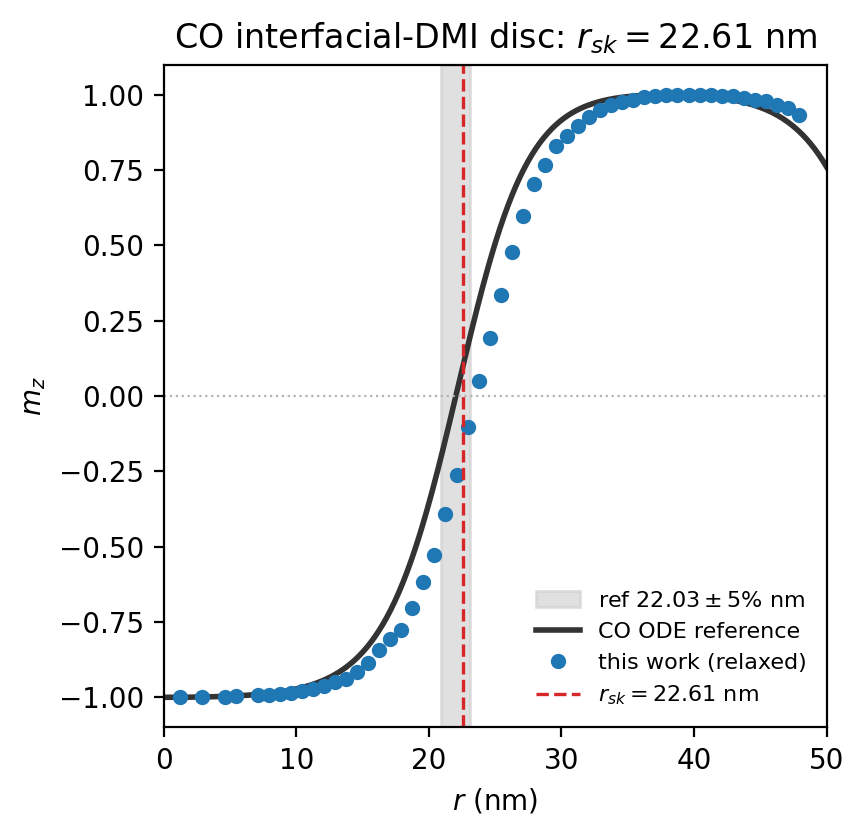
\includegraphics[width=0.56\textwidth]{fig01_co_dmi.png}
\caption{Relaxed radial profile $m_z(r)$ (this work, free-BC disc,
production \texttt{effective\_field}+\texttt{relax}) against the
CO ODE reference. Measured $r_{sk}=22.61$ nm (2.62\%, tol 5\%);
outward-N\'eel chirality confirmed.}
\end{figure}

\begin{figure}[htbp]
\centering
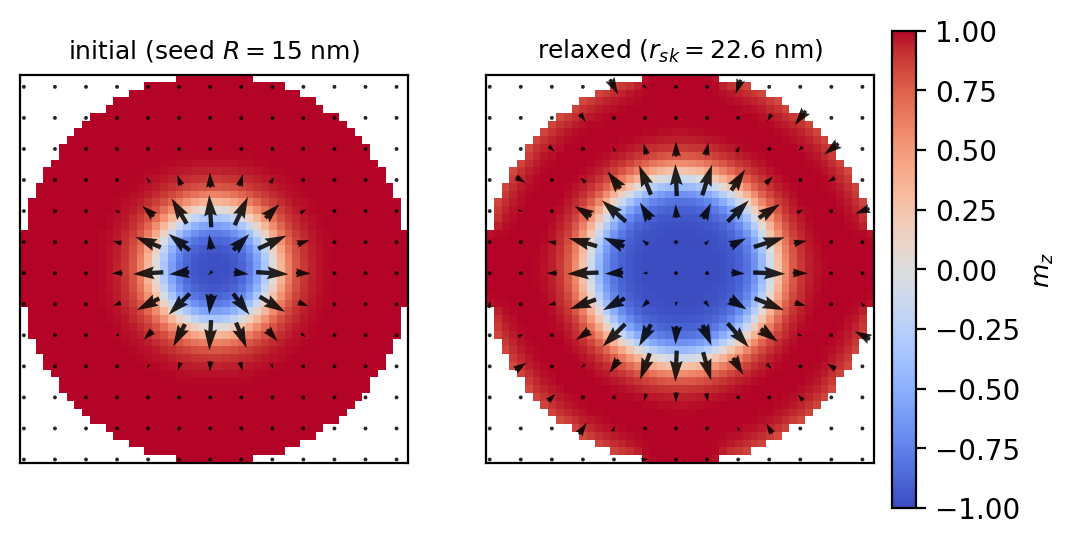
\includegraphics[width=0.78\textwidth]{fig01_co_config.png}
\caption{Configurations: the seeded skyrmion ($R=15$ nm) relaxes to
the equilibrium isolated skyrmion ($r_{sk}=22.6$ nm) in the disc.
Colour is $m_z$; arrows the in-plane components (outward N\'eel).}
\end{figure}

\paragraph{Behaviour / status.} \PASS. $r_{sk}=22.61$ nm (2.62\%
vs theory); profile RMS $0.11$ (tol 15\%). \textbf{Limitations:}
the profile-RMS tolerance is $15\%$ because a 5\%-level $r_{sk}$
shift on a $\Delta\!\approx\!5.7$ nm wall already gives RMS
${\sim}0.1$ (wall-position dominated; the published OOMMF/mumax3
runs show the same). The DMI boundary-condition sign follows
mumax3 (opposite to RT 2013 Eq.\,6) with identical bulk chirality.

% ============================================================
\clearpage
\section{Bogdanov--Hubert / RT 2013 isolated-skyrmion profile}
\label{sec:bh}

\paragraph{Reference.} Rohart \& Thiaville, \emph{PRB} 88, 184422
(2013), Eq.\,18: $R_s=\Delta/\sqrt{2(1-D/D_c)}$ (infinite film, no
demag, $K$ already $K_{\rm eff}$). $R_{s,\rm ref}=9.463$ nm at
$D/D_c=0.825$.

\begin{table}[htbp]
\centering
\caption{Material parameters (reference vs this work).}
\begin{tabular}{@{}lll@{}}
\toprule
Quantity & Reference (RT 2013) & This work \\
\midrule
Exchange $A$        & 16 pJ/m        & 16 pJ/m \\
$K_{\rm eff}$       & 0.51 MJ/m$^3$  & 0.51 MJ/m$^3$ \\
$\mu_0 M_s$         & 1.1 T          & 1.1 T \\
DMI $D$             & 3 mJ/m$^2$     & 3 mJ/m$^2$ ($D/D_c{=}0.825$)\\
$\Delta=\sqrt{A/K}$ & 5.60 nm        & 5.60 nm \\
Cell / lattice      & ---            & 1 nm, $96^2$ (PBC) \\
Demagnetisation     & off            & off \\
\bottomrule
\end{tabular}
\end{table}

\begin{figure}[htbp]
\centering
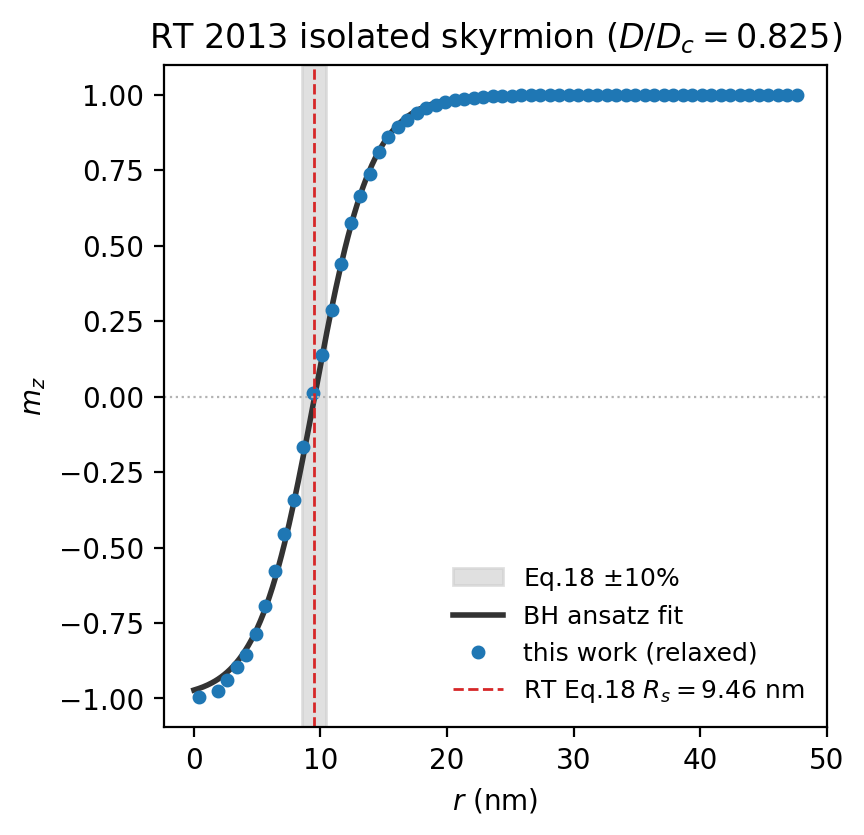
\includegraphics[width=0.56\textwidth]{fig02_bh_profile.png}
\caption{Relaxed $m_z(r)$ (this work) with a Bogdanov--Hubert
ansatz fit; the dashed line marks RT Eq.\,18 $R_s=9.46$ nm.
Measured $R_s=9.32$ nm (1.50\%, tol 10\%), shape RMS $0.012$.}
\end{figure}

\begin{figure}[htbp]
\centering
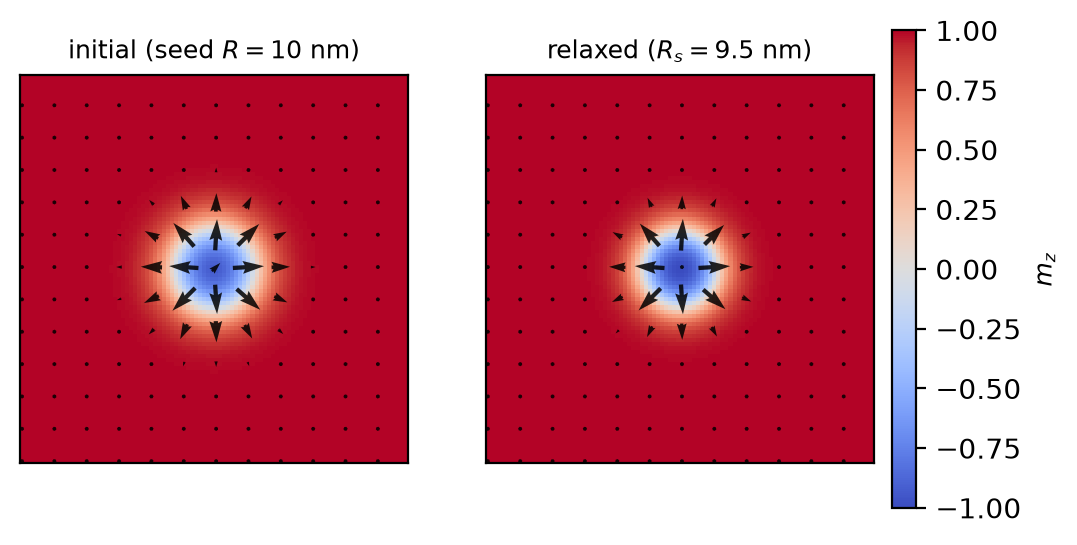
\includegraphics[width=0.78\textwidth]{fig02_bh_config.png}
\caption{Configurations: seeded skyrmion ($R=10$ nm) $\to$ relaxed
isolated skyrmion ($R_s=9.3$ nm) in the PBC box.}
\end{figure}

\paragraph{Behaviour / status.} \PASS. Only $R_s$ is gated; the
fitted wall width $\Delta_{\rm fit}=4.53$ nm differs from the
thin-wall $\sqrt{A/K}$ because Eq.\,18 is itself an asymptotic
approximation (curvature-corrected core). Profile RMS reported,
not gated.

% ============================================================
\clearpage
\section{NIST muMAG Standard Problem \#4 (Permalloy, Field 1)}
\label{sec:sp4}

\paragraph{Reference.} NIST muMAG SP\#4 (Eicke \& McMichael). Ten
contributed solutions agree to ${\sim}3\%$; the first
$\langle m_x\rangle{=}0$ crossing under Field 1 is at
${\approx}136$ ps.

\begin{table}[htbp]
\centering
\caption{Material parameters (reference vs this work).}
\begin{tabular}{@{}lll@{}}
\toprule
Quantity & Reference (NIST) & This work \\
\midrule
Exchange $A$    & 13 pJ/m       & 13 pJ/m \\
$M_s$           & 0.8 MA/m      & 0.8 MA/m \\
Anisotropy $K$  & 0             & 0 \\
$\alpha$        & 0.02          & 0.02 \\
$\gamma$        & $1.76\times10^{11}$ & $1.76\times10^{11}$ \\
Geometry        & $500{\times}125{\times}3$ nm
                & same (rect mask) \\
Field 1 $\mu_0H$& $(-24.6,4.3,0)$ mT & same \\
Cell            & ${\sim}2.5$ nm & 2.5 nm \\
Demagnetisation & full          & Newell free-BC (single layer) \\
\bottomrule
\end{tabular}
\end{table}

\begin{figure}[htbp]
\centering
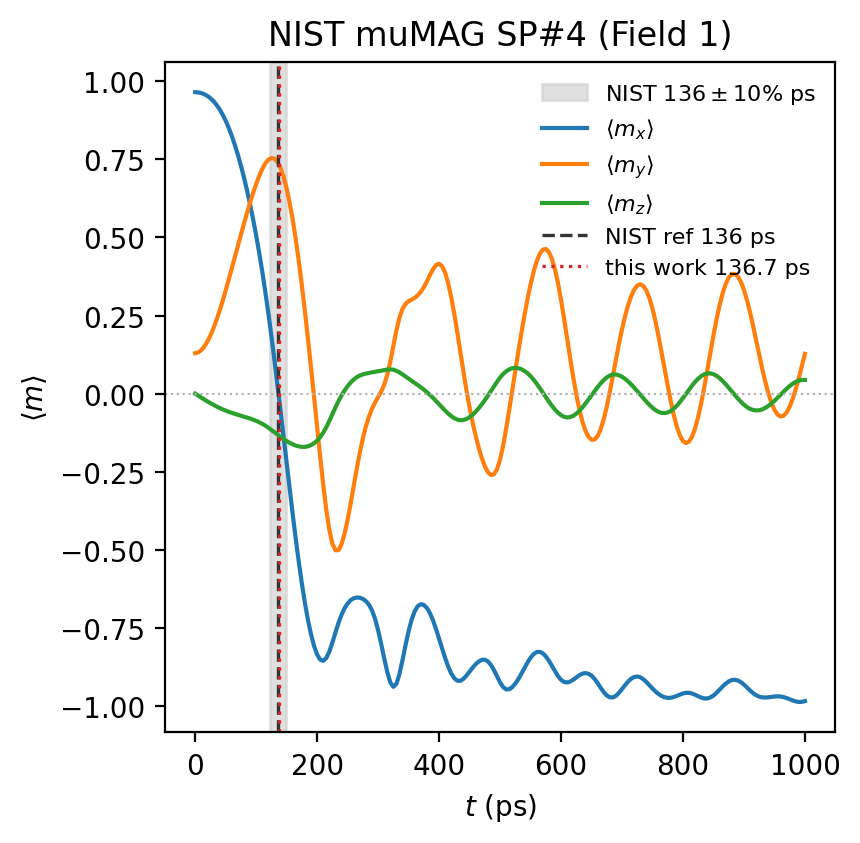
\includegraphics[width=0.58\textwidth]{fig03_sp4.png}
\caption{This work: spatially-averaged $\langle m\rangle(t)$ under
Field 1 (single FM layer, Newell free-BC demag, production
\texttt{rk4\_step\_single}). First $\langle m_x\rangle{=}0$ crossing
at $136.7$ ps (0.49\% vs the NIST ${\approx}136$ ps).}
\end{figure}

\begin{figure}[htbp]
\centering
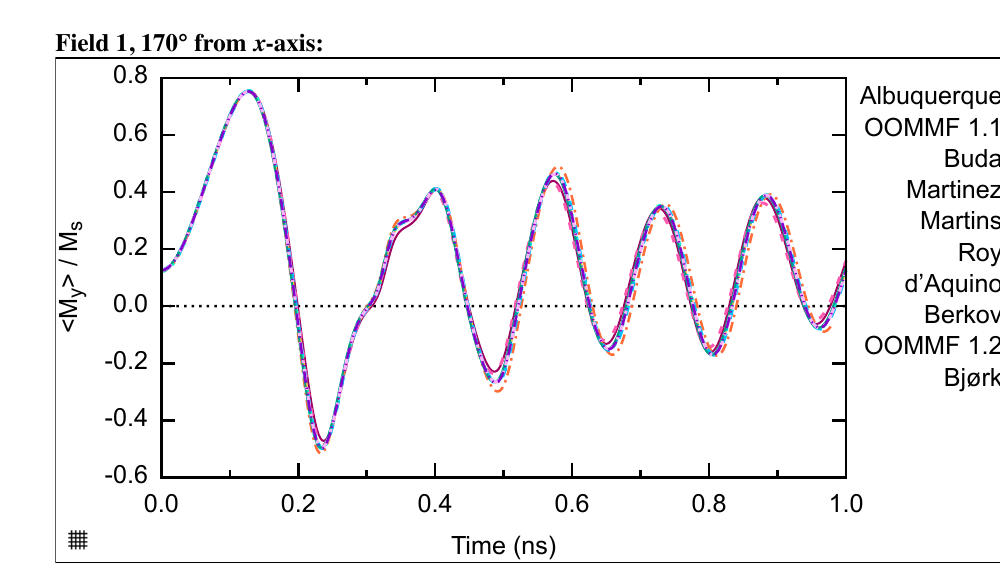
\includegraphics[width=\textwidth]{ref_nist_sp4.png}
\caption{Reference: NIST muMAG SP\#4 results,
$\langle M_y\rangle/M_s$ under Field 1, the ten contributed
solutions (agree to ${\sim}3\%$). Our $\langle m_y\rangle$ peaks
${\approx}0.75$ at ${\sim}130$ ps, matching the curve shape and the
first zero-crossing.}
\end{figure}

\begin{figure}[htbp]
\centering
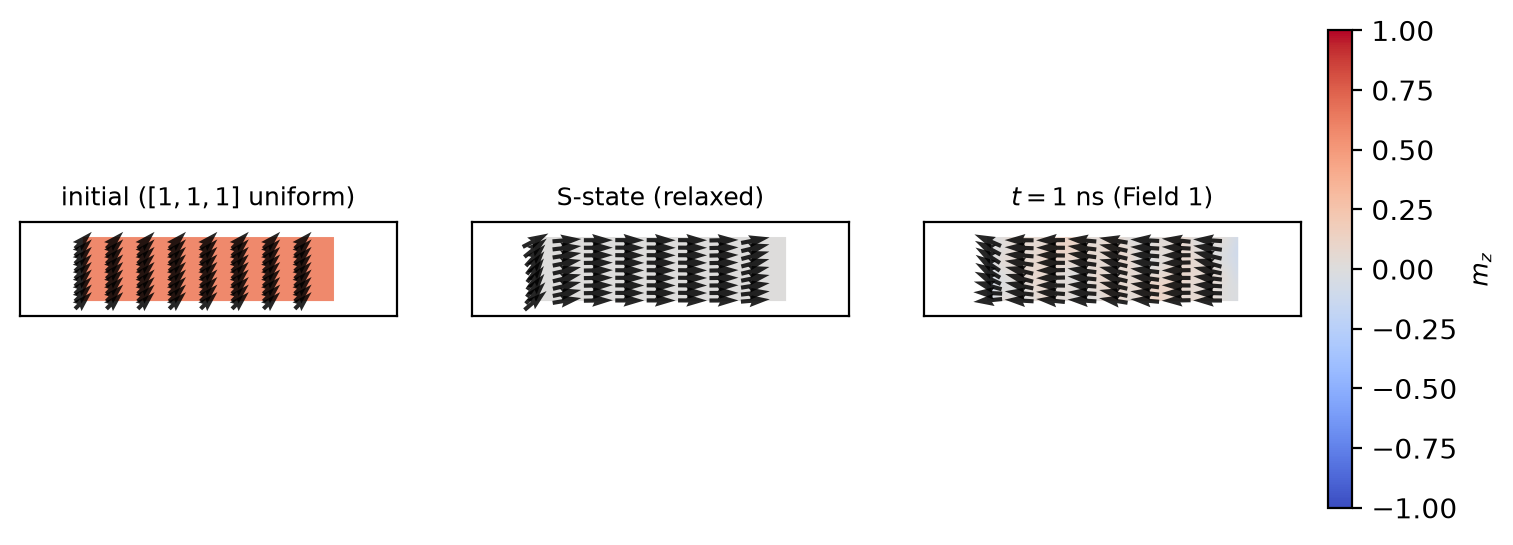
\includegraphics[width=\textwidth]{fig03_sp4_config.png}
\caption{Configurations: the uniform $[1,1,1]$ start relaxes to the
S-state, which under Field 1 reverses; the snapshot at $t=1$ ns
shows the partially-reversed magnetisation.}
\end{figure}

\paragraph{Behaviour / status.} \PASS. Crossing at $136.7$ ps
(0.49\%, tol 10\%). \textbf{Limitations:} cell $2.5$ nm (the 10\%
gate absorbs the discretisation). An earlier wrong result
(${\sim}290$ ps) came from a dummy SAF bottom layer adding spurious
inter-layer demag; fixed by evolving a genuine single layer via
\texttt{rk4\_step\_single}.

% ============================================================
\clearpage
\section{NIST muMAG Standard Problem \#5 (Zhang--Li STT vortex)}
\label{sec:sp5}

\paragraph{Reference.} Najafi \emph{et al.} 2009 (SP\#5 proposal):
steady-state vortex-core displacement $\Delta x=-1.2$ nm,
$\Delta y=-14.7$ nm for $\xi=0.05$.

\begin{table}[htbp]
\centering
\caption{Material parameters (reference vs this work).}
\begin{tabular}{@{}lll@{}}
\toprule
Quantity & Reference (Najafi 2009) & This work \\
\midrule
Material        & Permalloy          & Permalloy \\
Geometry        & $100{\times}100{\times}10$ nm & same \\
STT model       & Zhang--Li          & Zhang--Li (Thiaville form)\\
$\xi$ (non-adiab.) & 0.05            & 0.05 \\
$u_T$           & $-72.17$ m/s       & $-72.17$ m/s \\
Drive window    & 8 ns               & 8 ns \\
\bottomrule
\end{tabular}
\end{table}

\begin{figure}[htbp]
\centering
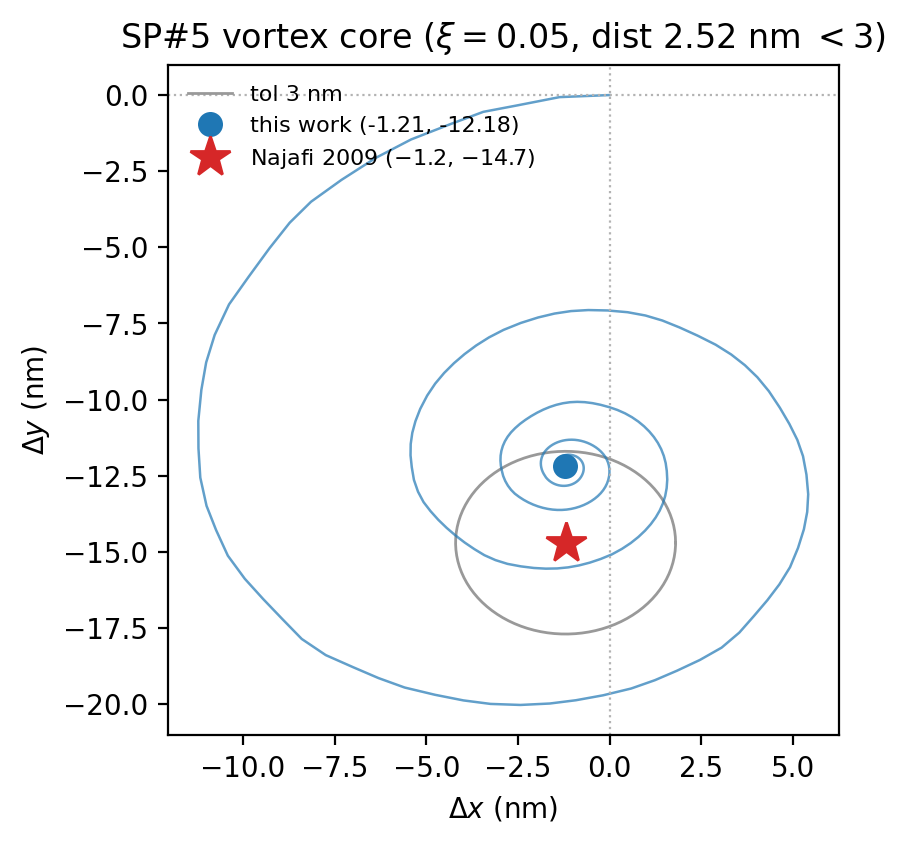
\includegraphics[width=0.56\textwidth]{fig04_sp5_trajectory.png}
\caption{Vortex-core displacement trajectory (this work) via the
production \texttt{zhang\_li\_torque}+\texttt{rk4\_step\_single};
the star marks the Najafi 2009 steady-state target.}
\end{figure}

\begin{figure}[htbp]
\centering
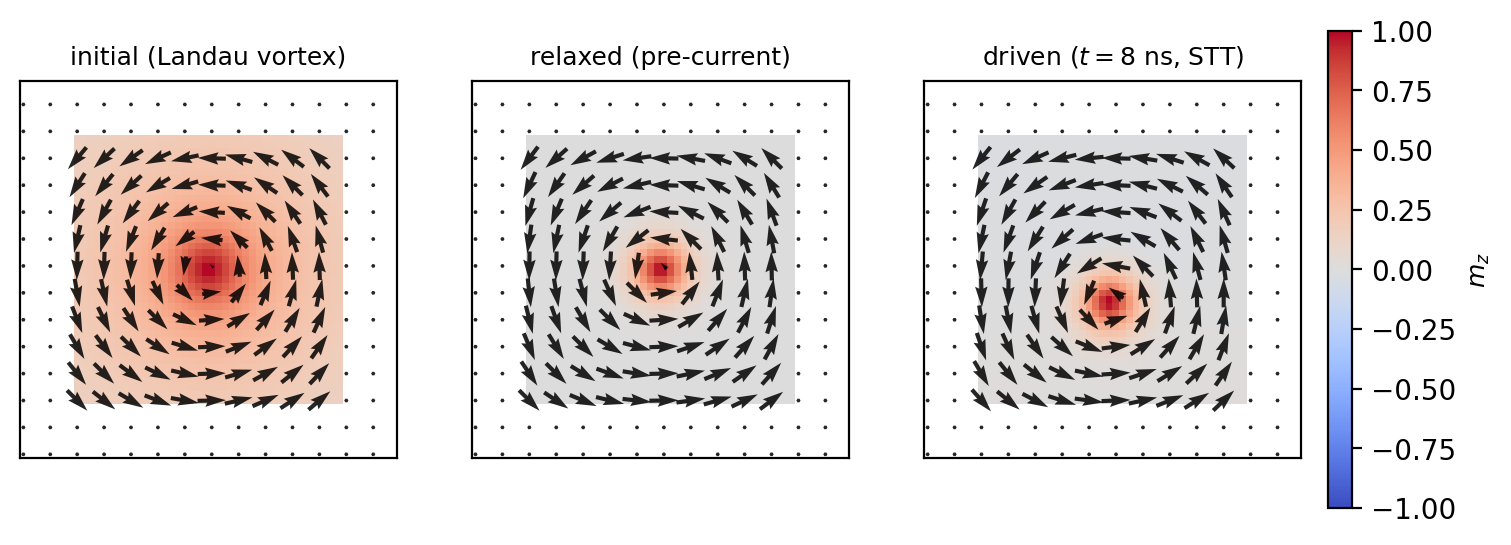
\includegraphics[width=\textwidth]{fig04_sp5_config.png}
\caption{Configurations: the Landau-vortex seed relaxes
(pre-current), then the Zhang--Li STT drives the core to its
steady displaced position after 8 ns.}
\end{figure}

\paragraph{Behaviour / status.} \PASS. $\Delta x=-1.21$ nm
(${\approx}0.01$ nm off), $\Delta y=-12.18$ nm (${\approx}2.5$ nm
off), total distance $2.52$ nm (tol 3 nm). \textbf{Limitations:}
$\Delta y$ is ${\sim}17\%$ short of $-14.7$ nm, attributed to the
$2.5$ nm grid and the 8 ns window not being fully settled; within
the 3 nm distance gate.

% ============================================================
\clearpage
\section{1D domain-wall width}
\label{sec:dw}

\paragraph{Reference.} Textbook 1D N\'eel/Bloch wall,
$\Delta=\sqrt{A/K_{\rm eff}}$ (universal). This benchmark proves
the production field+integrator reproduce the
exchange--anisotropy balance.

\begin{table}[htbp]
\centering
\caption{Parameters (the relation is universal; values arbitrary).}
\begin{tabular}{@{}lll@{}}
\toprule
Quantity & Reference & This work \\
\midrule
Exchange $A$   & ---  & 16 pJ/m \\
$K_{\rm eff}$  & ---  & 0.1 MJ/m$^3$ \\
$M_s$          & ---  & 1.43 MA/m \\
$\Delta_{\rm analytic}$ & $\sqrt{A/K}$ & 12.6491 nm \\
Lattice        & ---  & $401{\times}8$, $a=1$ nm, pinned ends \\
\bottomrule
\end{tabular}
\end{table}

\begin{figure}[htbp]
\centering
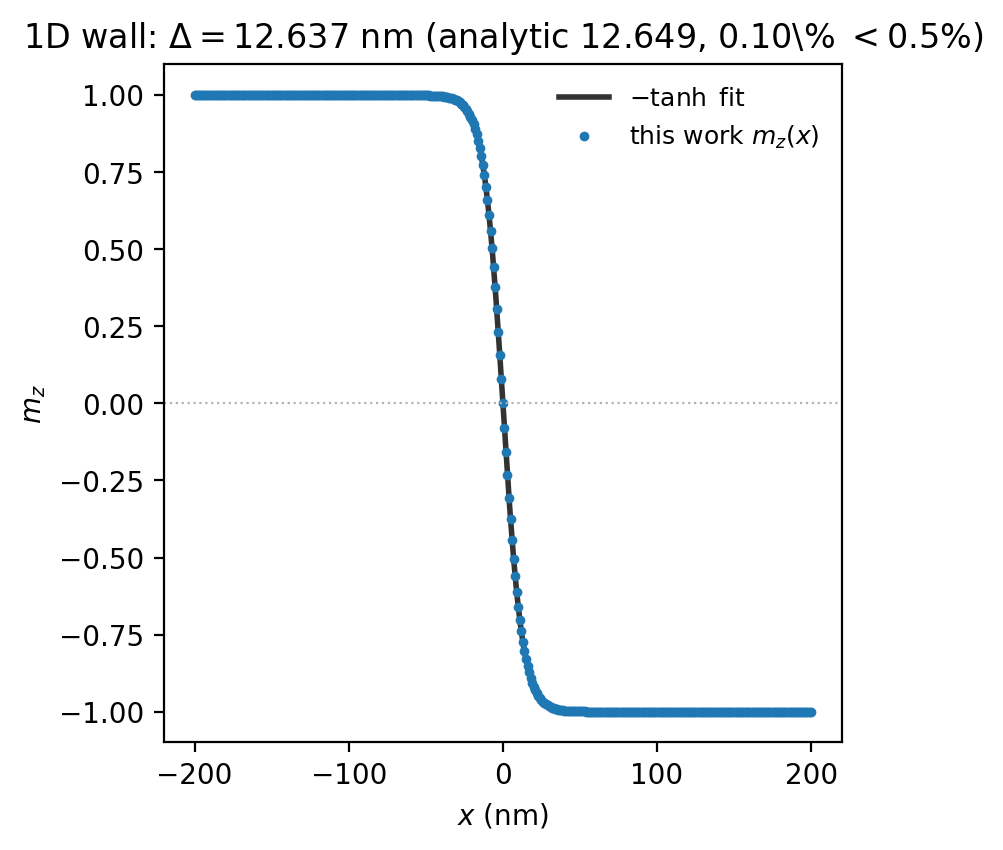
\includegraphics[width=0.56\textwidth]{fig11_dw_profile.png}
\caption{Relaxed $m_z(x)$ (production \texttt{effective\_field}
+\texttt{rk4\_step\_single}, $D{=}0$, no demag) fit to
$-\tanh((x-x_0)/\Delta)$.}
\end{figure}

\begin{figure}[htbp]
\centering
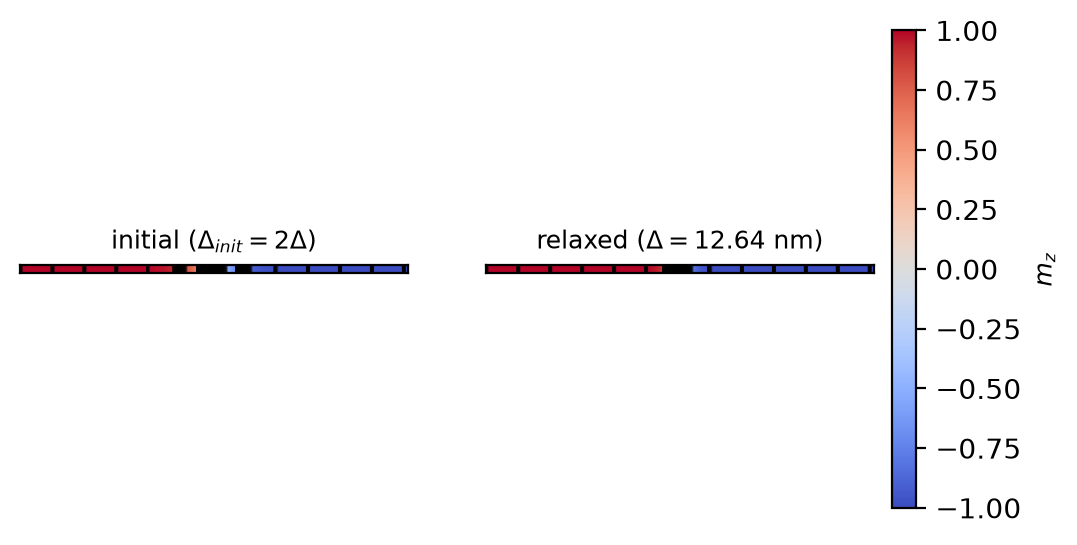
\includegraphics[width=0.95\textwidth]{fig11_dw_config.png}
\caption{Configurations ($m_z$ on the $401\times8$ strip): the
deliberately-wide tanh seed ($\Delta_{init}=2\Delta$) relaxes to the
equilibrium wall; pinned $\pm z$ end columns hold the single wall.}
\end{figure}

\paragraph{Behaviour / status.} \PASS. $\Delta=12.637$ nm
(0.095\%, tol 0.5\%). No material deviation.

% ============================================================
\clearpage
\section{Uniform-mode FMR frequency}
\label{sec:fmr}

\paragraph{Reference.} Macrospin FMR, $f=(\gamma/2\pi)H_K$ with
$H_K=2K_{\rm eff}/M_s$ (no Zeeman, no DMI, no demag).

\begin{table}[htbp]
\centering
\caption{Material parameters (reference vs this work).}
\begin{tabular}{@{}lll@{}}
\toprule
Quantity & Reference & This work \\
\midrule
Exchange $A$  & ---  & 16 pJ/m \\
$K_{\rm eff}$ & ---  & 0.5 MJ/m$^3$ \\
$M_s$         & ---  & 0.8 MA/m \\
$\gamma$      & ---  & $1.76\times10^{11}$ \\
$f_{\rm analytic}=\gamma H_K/2\pi$ & ${\approx}35$ GHz
              & ${\approx}35$ GHz \\
\bottomrule
\end{tabular}
\end{table}

\begin{figure}[htbp]
\centering
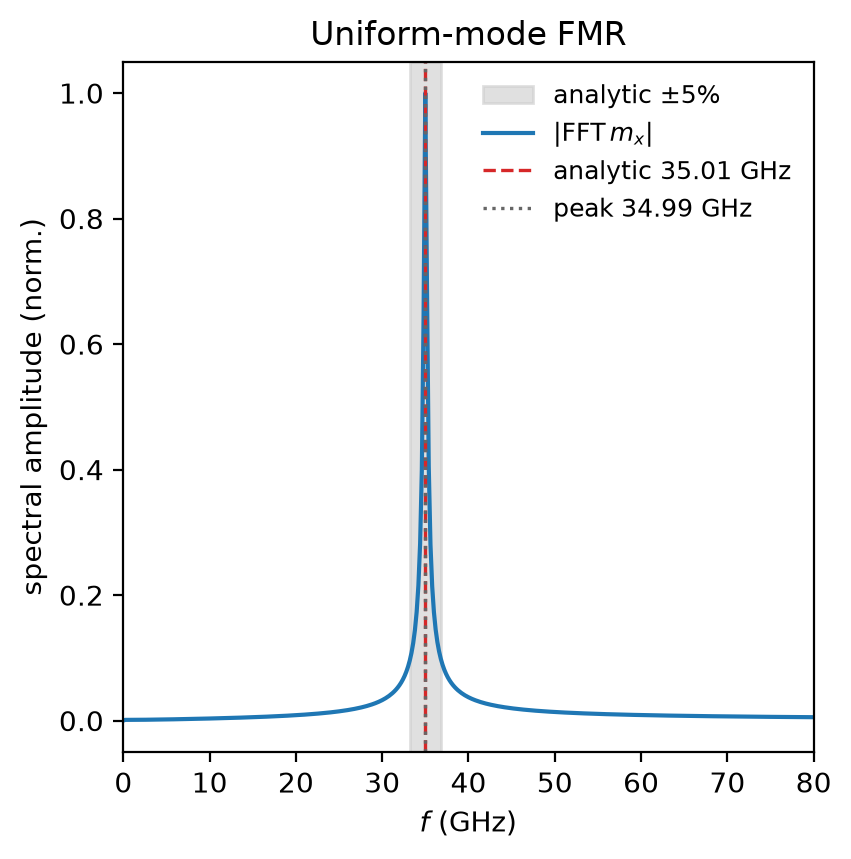
\includegraphics[width=0.56\textwidth]{fig12_fmr.png}
\caption{FFT of the spatially-averaged $m_x(t)$ precession; the
peak matches the analytic uniform-mode frequency.}
\end{figure}

\paragraph{Behaviour / status.} \PASS. FFT peak within $<5\%$.
The configuration is a spatially-uniform macrospin (uniform $+z$
with a small in-plane tilt) precessing coherently, so there is no
spatial texture to display; the relaxed value is the FFT peak
frequency compared to the $\pm5\%$ band in the figure.
\textbf{Limitations:} this validates the $k{=}0$ uniform-mode
frequency only, not a full spin-wave dispersion $\omega(k)$ --- the
cleanest analytic anchor for the field+integrator.

% ============================================================
\clearpage
\section{Thiele $v_{SOT}(R/\Delta)$ and $v_{TSH}$ vs Pham 2024
Fig.\,S49}
\label{sec:thiele}

\paragraph{Reference.} Pham \emph{et al.}, \emph{Fast
current-induced skyrmion motion in synthetic antiferromagnets}
(2024), Fig.\,S49 and supplement \S1.7. Two closed forms vs
$R/\Delta$ at fixed $\Delta=24.5$ nm: the SOT speed
$v_{SOT}=\pi H_{DL} R\gamma/[2\alpha(R/\Delta+\Delta/R)]$ and the
topological-spin-Hall speed $v_{TSH}$ ($\lambda^2\in\{3,50\}$
nm$^2$).

\begin{table}[htbp]
\centering
\caption{Parameters (Set B; reference vs this work).}
\begin{tabular}{@{}lll@{}}
\toprule
Quantity & Reference (Pham, Set B) & This work \\
\midrule
$\alpha$        & 0.216             & 0.216 \\
$\gamma$        & 175.9 GHz/T       & 175.9 GHz/T \\
DMI $D$         & 0.62 mJ/m$^2$     & 0.62 mJ/m$^2$ \\
$\Delta$ (fixed)& 24.5 nm           & 24.5 nm \\
$R/\Delta$      & 1--5 (imposed)    & 1--5 (imposed) \\
$\lambda^2$     & 3, 50 nm$^2$      & 3, 50 nm$^2$ \\
$J_0$ (curves)  & $8\times10^{11}$  & $8\times10^{11}$ \\
LLGS spot-check & ---               & $1\times10^{11}$ \\
\bottomrule
\end{tabular}
\end{table}

\begin{figure}[htbp]
\centering
\begin{subfigure}{0.49\textwidth}\centering
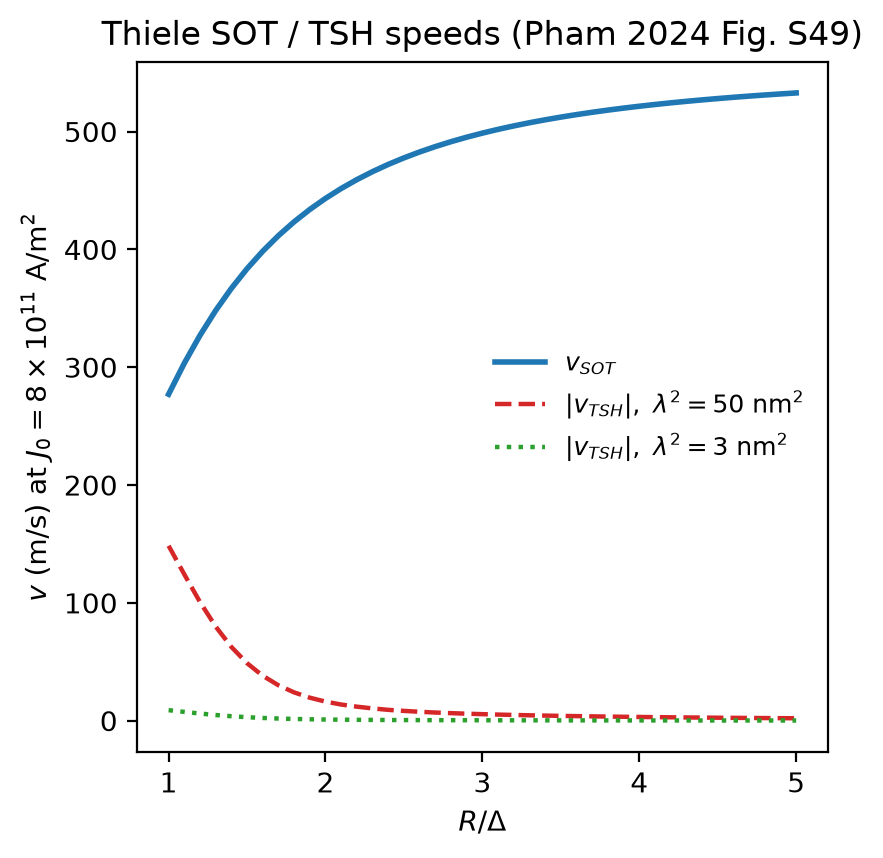
\includegraphics[width=\textwidth]{fig10_thiele.png}
\caption{This work: production \texttt{sot\_thiele\_speed} and
\texttt{tsh\_thiele\_speed} vs $R/\Delta$.}
\end{subfigure}\hfill
\begin{subfigure}{0.49\textwidth}\centering
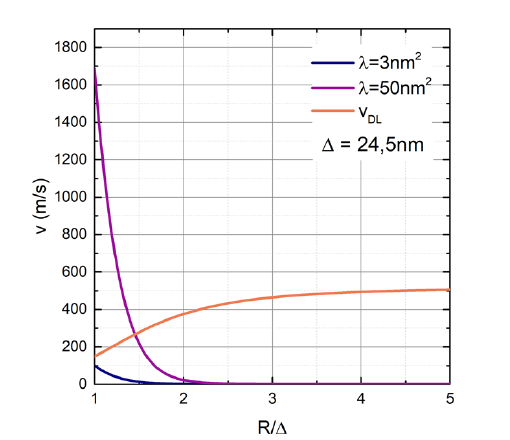
\includegraphics[width=\textwidth]{ref_pham_s49.png}
\caption{Reference: Pham 2024 Fig.\,S49 ($v_{DL}$ in orange,
$v_{TSH}$ for $\lambda^2{=}3,50$ nm$^2$).}
\end{subfigure}
\caption{Thiele SOT/TSH speeds. $v_{SOT}$ reproduces S49
quantitatively (rises and saturates at ${\approx}530$ m/s vs the
paper's ${\approx}500$); $v_{TSH}$ reproduces the S49 \emph{shape}
(sub-dominant, decays with $R/\Delta$, rises sharply as
$R/\Delta\!\to\!1$, exactly $\propto\lambda^2$) but its absolute
small-$R/\Delta$ magnitude is grid-cutoff dependent (see below).}
\end{figure}

\begin{figure}[htbp]
\centering
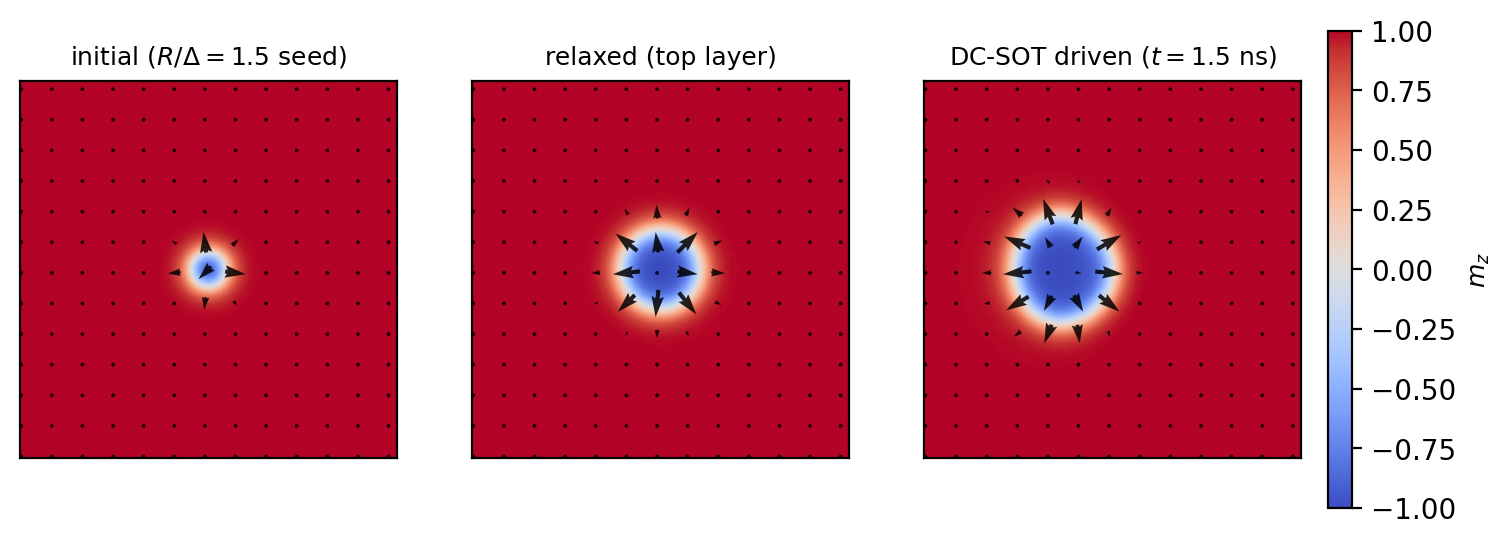
\includegraphics[width=\textwidth]{fig10_thiele_config.png}
\caption{LLGS spot-check configurations (top layer $m_z$): the
$R/\Delta=1.5$ SAF seed relaxes, then a DC SOT pulse
($J_0=1\times10^{11}$) translates it rigidly over 1.5 ns (no
skyrmion-Hall deflection, as expected for a compensated SAF).}
\end{figure}

\paragraph{Behaviour / status.} \PASS. Analytic gate matches the
independently-derived closed form to $2\times10^{-16}$;
$v_{SOT}$ monotone/saturating and quantitatively matching the
paper's saturation speed; $v_{TSH}\propto\lambda^2$ exactly.
A micromagnetic LLGS spot-check (relax one SAF skyrmion, drive with
DC SOT) gives $v_{\rm meas}$ vs Thiele $9.9\%$ (gate $15\%$) and
drive-induced deformation $4\%$ (rigid). An earlier revision quoted
$1.5\%$: that run used a nonstandard SOT torque with a normalised
polarisation vector, whose ${\sim}{+}10\%$ drive inflation
coincidentally cancelled the demag-geometry offset of the
asymptotic closed form. With the corrected (standard Slonczewski)
torque, a five-number decomposition on a demag-free profile shows
the closed form within $1.7\%$ of the exact Thiele integral, the
measured LLGS within $2.6\%$ of the closed form, and the
legacy-to-standard velocity ratio $1.100$ in both the projected
force and the measured speed; the residual $9.9\%$ on the
Newell-demag geometry reflects that demag-dressed, still-creeping
profile, not the torque. \textbf{Limitations:} (i) Fig.\,S49 is an
analytic calculation (imposed $R/\Delta$, fixed $\Delta$). The spot
runs at $1\times10^{11}$ (the DC-pulse current of Fig.\,S47 where
the velocity plateaus), not the $8$--$8.9\times10^{11}$ of the
deformation study --- at that high current the paper itself
documents skyrmion expansion/elliptical deformation that breaks the
rigid-Thiele model. Rigidity is gated on the $J{=}0$-referenced
drive deformation, which cancels relaxation creep.
(ii) The \emph{absolute} $v_{TSH}$ near $R/\Delta\!\to\!1$ is below
the paper's ($|v_{TSH}|\!\approx\!148$ m/s here vs ${\sim}1600$ in
S49 at $R/\Delta{=}1$, $\lambda^2{=}50$ nm$^2$): $v_{TSH}\propto
\int N_{xy}^2$ is logarithmically sensitive to the small-$r$ UV
cutoff (the lattice spacing) and to the integration box, so its
small-skyrmion magnitude is mesh-dependent. The benchmark therefore
gates the $v_{TSH}$ \emph{scaling} ($\propto\lambda^2$) and the
$v_{SOT}$ closed form, not the $v_{TSH}$ absolute --- consistent
with S49's own point that the motion is SOT-dominated and the TSH
term a small correction.

% ============================================================
\clearpage
\section{G\"ung\"ord\"u 2016 phase-boundary overlay}
\label{sec:gungordu}

\paragraph{Reference.} G\"ung\"ord\"u \emph{et al.} 2016, Fig.\,3:
phase diagram in the dimensionless plane
($a_s=A_sJ/D^2$, $h_g=HJ/D^2$) with FM / SkX / SP (spiral) / SC
regions.

\begin{table}[htbp]
\centering
\caption{Mapping and sweep parameters.}
\begin{tabular}{@{}lll@{}}
\toprule
Quantity & Reference (G\"ung\"ord\"u) & This work \\
\midrule
Plane    & $(a_s,h_g)$ dimensionless & same (mapped) \\
Anisotropy & $A_s$ & $K=-A_{s,\rm phys}$ (demag off) \\
DMI $D$  & --- & 1.5 mJ/m$^2$ \\
Lattice  & variational cell & $64^2$, $a=5$ nm (fixed) \\
Grid     & --- & $50{\times}50$, 4 candidate ICs \\
Demag.   & --- & off \\
\bottomrule
\end{tabular}
\end{table}

\begin{figure}[htbp]
\centering
\begin{subfigure}{0.52\textwidth}\centering
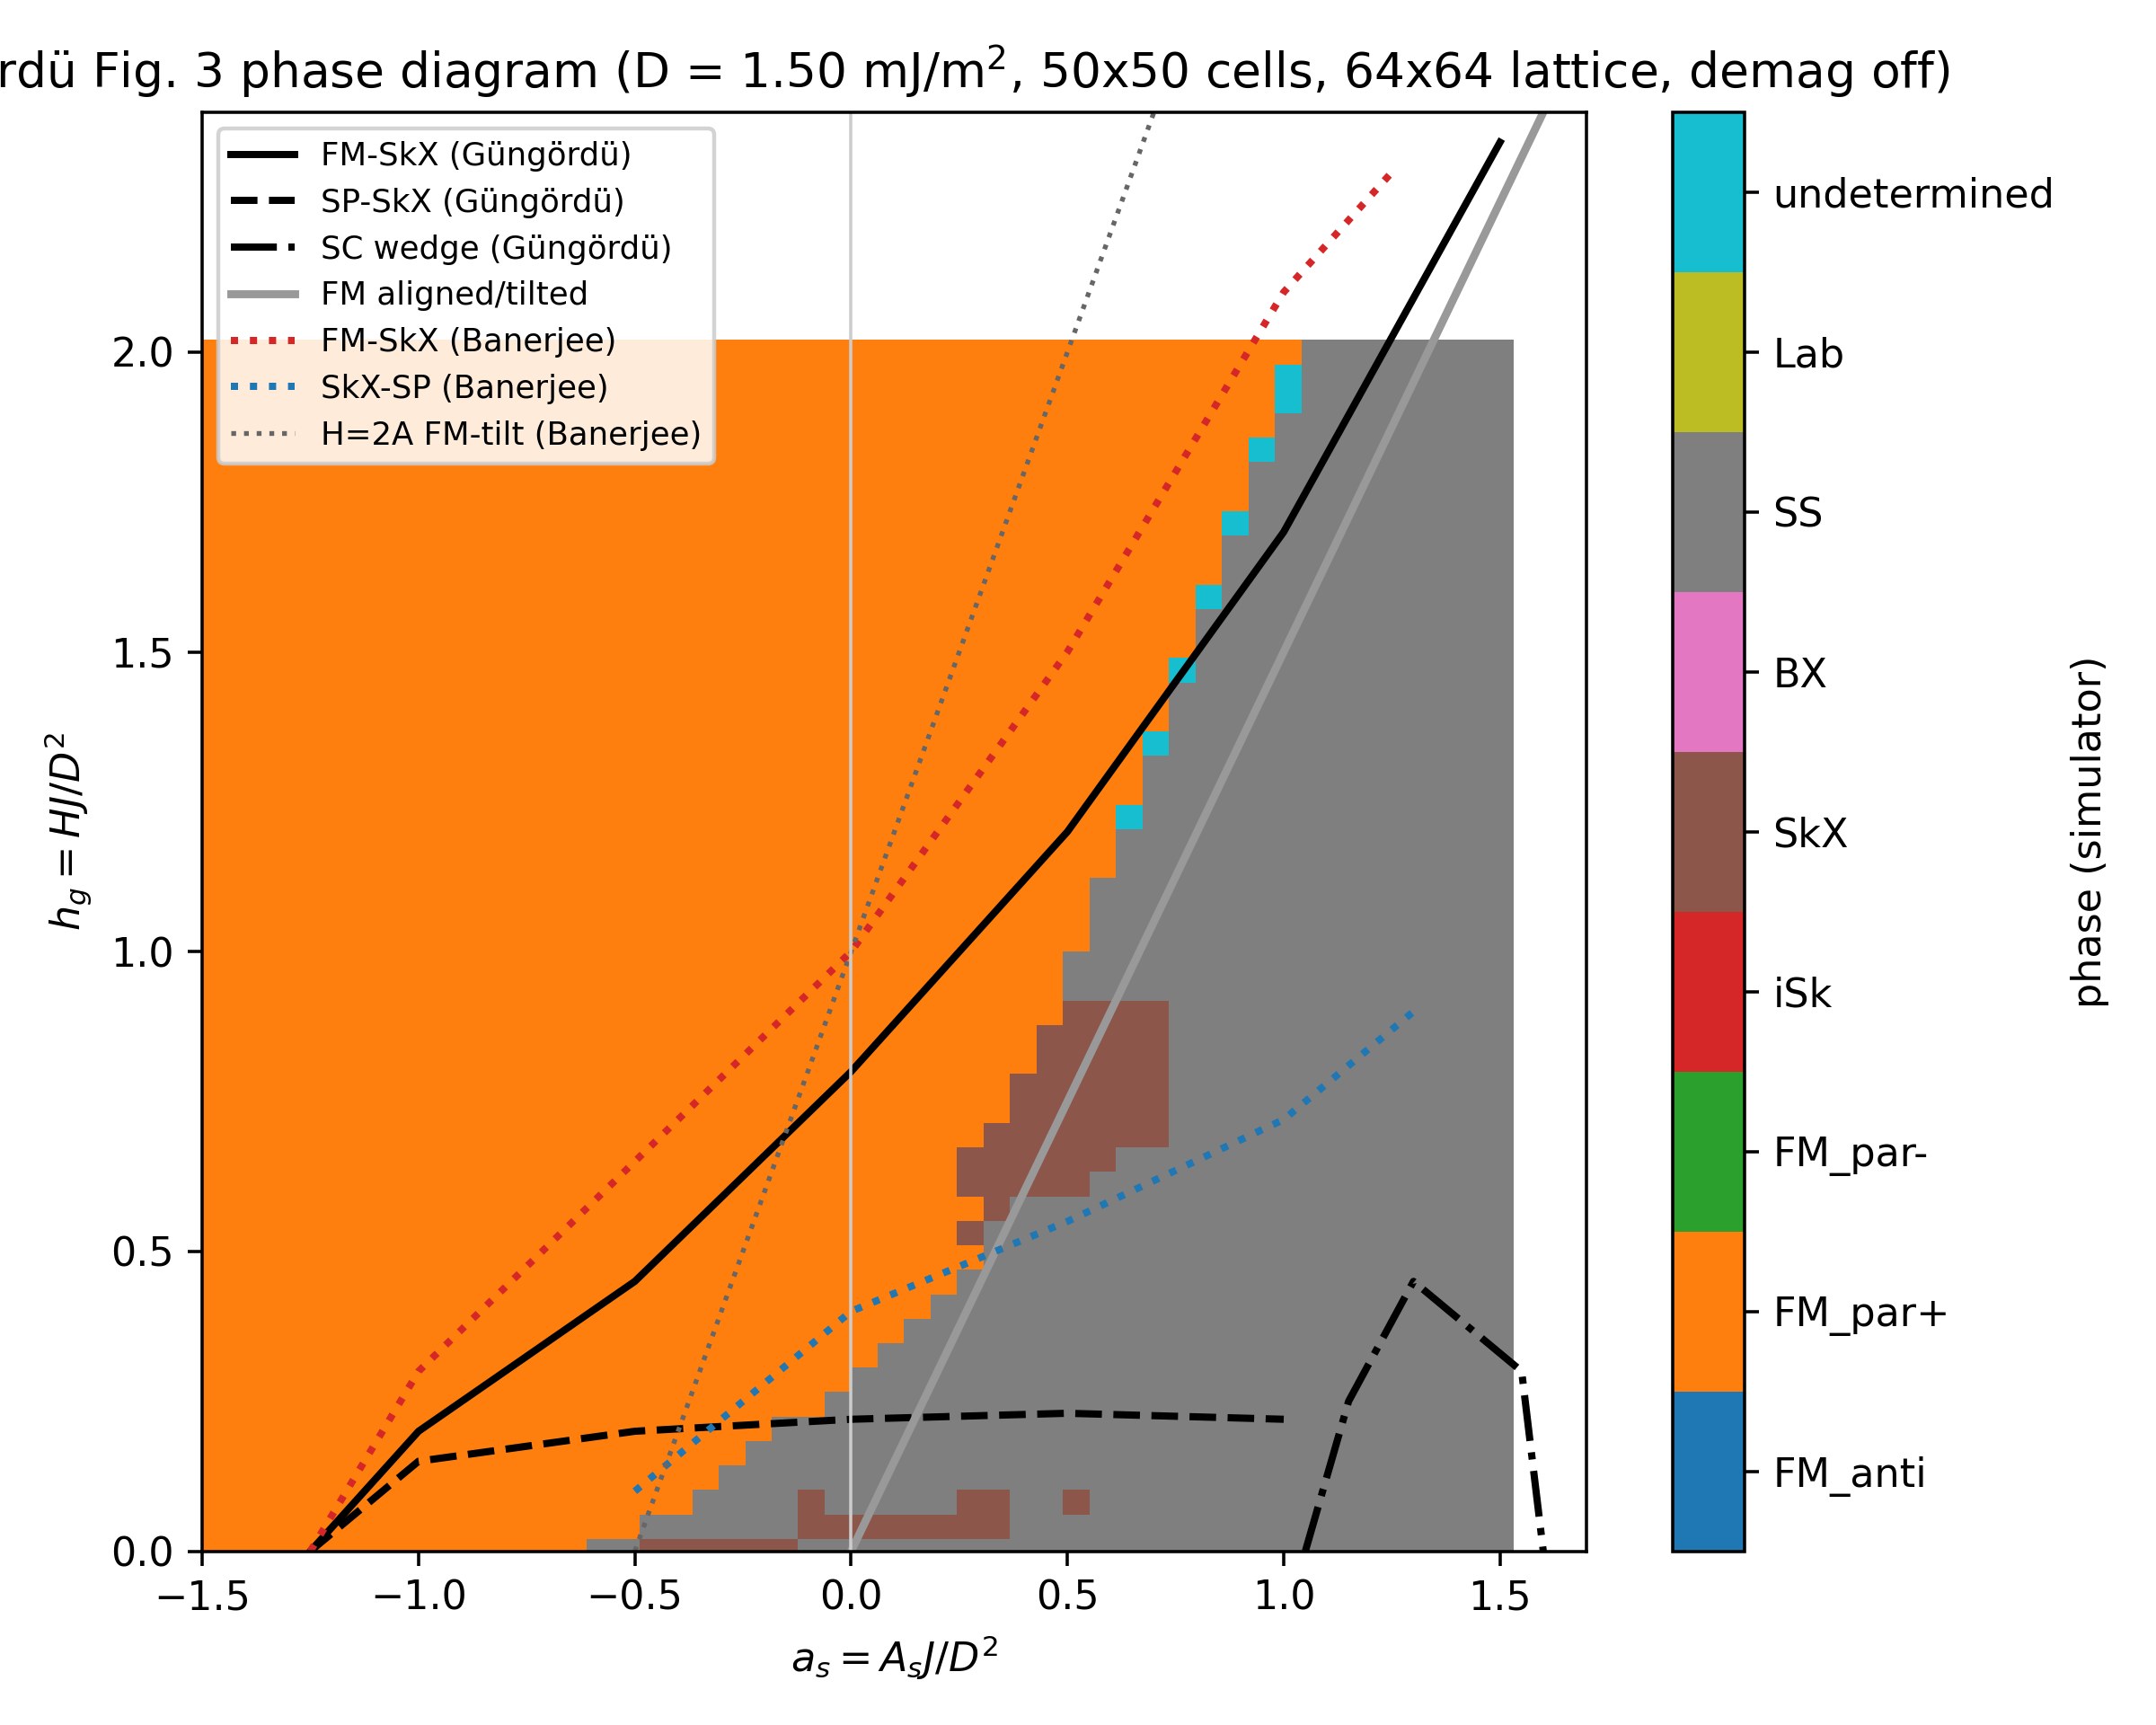
\includegraphics[width=\textwidth]{gungordu_phase_overlay.png}
\caption{This work: minimum-energy ground state over four candidate
initial conditions (FM / stripe / sk-lattice / sq-lattice).}
\end{subfigure}\hfill
\begin{subfigure}{0.46\textwidth}\centering
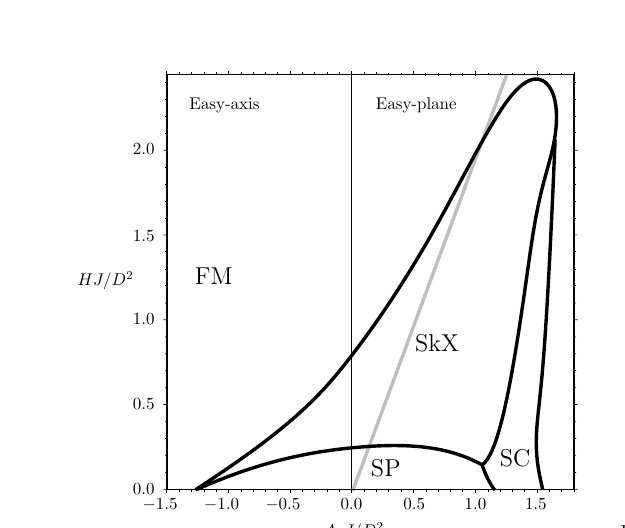
\includegraphics[width=\textwidth]{ref_gungordu_fig3.png}
\caption{Reference: G\"ung\"ord\"u 2016 Fig.\,3, zero-temperature
phase diagram ($HJ/D^2$ vs $A_sJ/D^2$) with FM / SkX / SP / SC
regions.}
\end{subfigure}
\caption{G\"ung\"ord\"u phase diagram. Our fixed-grid sweep
recovers the FM region and a modulated easy-plane region but
under-resolves the SkX lens (see below).}
\end{figure}

\begin{figure}[htbp]
\centering
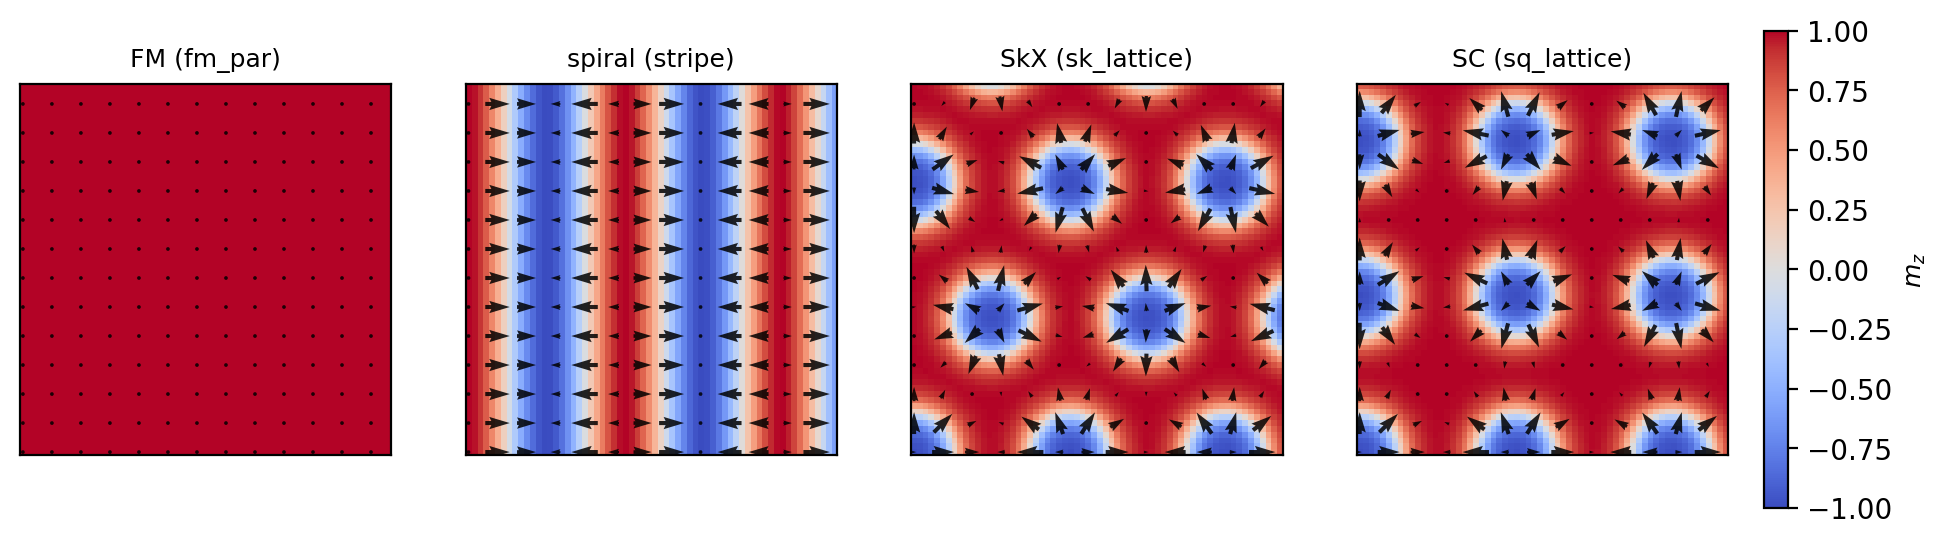
\includegraphics[width=\textwidth]{fig05_gungordu_config.png}
\caption{The four candidate initial textures the sweep relaxes and
compares by energy at each $(a_s,h_g)$ point: parallel FM, spin
spiral (SP), hexagonal skyrmion lattice (SkX), square lattice (SC).
The min-energy winner defines the ground state.}
\end{figure}

\paragraph{Behaviour / status.} \QUAL. The FM region and a
modulated easy-plane region are reproduced, but that region is
${\sim}32\%$ spiral and only ${\sim}2.6\%$ SkX, whereas
G\"ung\"ord\"u has a large SkX lens.
\textbf{Limitations:} a hexagonal SkX tiles a $\sqrt3$ rectangular
cell, so a fixed \emph{square} grid can never be hex-commensurate;
the flexible 1D spiral relaxes lower and wins where SkX should.
G\"ung\"ord\"u optimise the unit-cell size variationally per phase;
a fixed-grid sweep structurally cannot. Two real bugs were fixed en
route: (i) anisotropy sign ($K=-A_{s,\rm phys}$ with demag off),
(ii) ground state taken as \emph{minimum energy} over ICs (strict
torque convergence had collapsed everything to FM).

% ============================================================
\clearpage
\section{Banerjee 2014 FM$\leftrightarrow$SkX critical field}
\label{sec:banerjee}

\paragraph{Reference.} Banerjee \emph{et al.}, \emph{PRX} 4,
031045 (2014), Fig.\,1(b): the FM$\leftrightarrow$SkX critical
field $h_c(a_s)$ in the same dimensionless plane,
$h_c\approx1.03$--$1.52$.

\begin{table}[htbp]
\centering
\caption{Parameters (post-processing of the \#5 sweep).}
\begin{tabular}{@{}lll@{}}
\toprule
Quantity & Reference (Banerjee) & This work \\
\midrule
Plane     & $(a_s,h_g)$        & same (\#5 sweep) \\
Procedure & --- & field at SkX$\to$FM flip at fixed $a_s$ \\
New sim   & --- & none (reuses \#5) \\
\bottomrule
\end{tabular}
\end{table}

\paragraph{Behaviour / status.} \FAIL\ (quantitative, documented).
$h_{c,\rm sim}\approx0.18$--$0.96$ vs Banerjee $1.03$--$1.52$
(37--82\% low, tol 20\%). \textbf{Limitations:} same root cause as
\S\ref{sec:gungordu} --- the fixed square grid under-stabilises SkX,
so it is destroyed by a lower field than the variational ansatz
predicts. The topology (FM/SP) is right; the SkX stability window
is not. The phase map is shared with \S\ref{sec:gungordu}.

% ============================================================
\clearpage
\section{RT 2013 Fig.\,4(d) confined-skyrmion radius}
\label{sec:confined}

\paragraph{Reference.} Rohart \& Thiaville 2013, Fig.\,4(d):
confined skyrmion radius in a finite dot vs $D/D_c$; read value
$R_s\approx25$ nm at $R_{\rm dot}=50$ nm, $D/D_c=1.25$.

\begin{table}[htbp]
\centering
\caption{Material parameters (reference vs this work).}
\begin{tabular}{@{}lll@{}}
\toprule
Quantity & Reference (RT 2013) & This work \\
\midrule
Exchange $A$    & 16 pJ/m        & 16 pJ/m \\
$K_{\rm eff}$   & 0.50 MJ/m$^3$  & 0.50 MJ/m$^3$ \\
$M_s$           & 1.1 MA/m       & 1.1 MA/m \\
DMI $D$         & 4.5 mJ/m$^2$   & 4.5 mJ/m$^2$ ($D/D_c{=}1.25$)\\
Dot radius      & 50 nm          & 50 nm \\
Cell / lattice  & ---            & 2 nm, $60^2$ (free-BC) \\
\bottomrule
\end{tabular}
\end{table}

\begin{figure}[htbp]
\centering
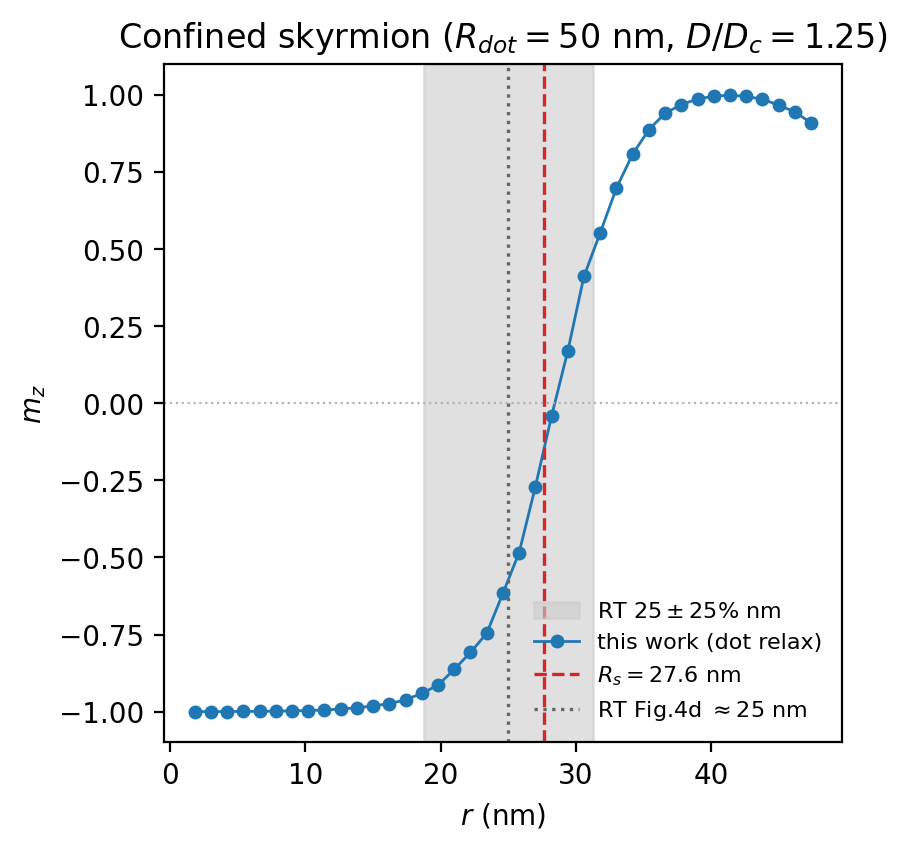
\includegraphics[width=0.56\textwidth]{fig07_confined_rt.png}
\caption{Relaxed $m_z(r)$ in the 50 nm dot (production
\texttt{relax}, single-layer free-BC mask); the dotted line is the
RT Fig.\,4(d) read value ${\approx}25$ nm.}
\end{figure}

\begin{figure}[htbp]
\centering
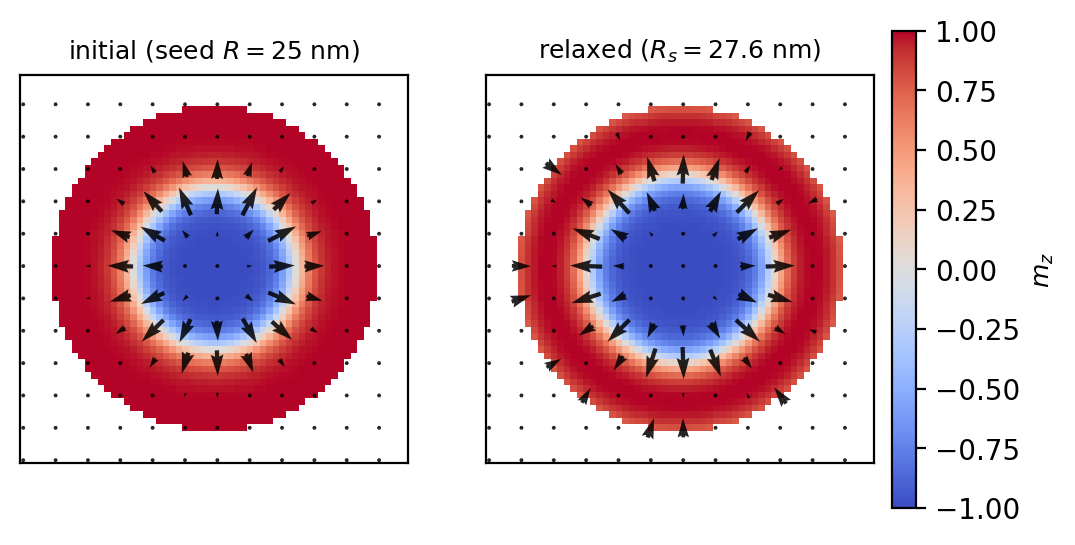
\includegraphics[width=0.78\textwidth]{fig07_confined_config.png}
\caption{Configurations: seeded skyrmion ($R=25$ nm) $\to$ relaxed
confined skyrmion ($R_s=27.6$ nm) in the 50 nm dot (free-BC mask).}
\end{figure}

\paragraph{Behaviour / status.} \PASS. $R_s=27.6$ nm (${\approx}10\%$,
tol 25\%). \textbf{Limitations:} Eq.\,18 (infinite-film) diverges
for $D\ge D_c$, so above threshold the dot radius alone sets $R_s$;
the comparison uses the Fig.\,4(d) read value with a loose
figure-read tolerance.

% ============================================================
\clearpage
\section{Tomasello 2018 skyrmion-size temperature scaling}
\label{sec:tomasello}

\paragraph{Reference.} R.\ Tomasello \emph{et al.}, \emph{PRB} 97,
060402(R) (2018), Fig.\,1(b): skyrmion diameter vs temperature in a
confined dot at $H=0/25/50$ mT. Temperature enters \emph{only}
through the reduced magnetisation $m(T)=M_s(T)/M_s(0)$, which scales
parameters by Callen--Callen exponents
$M_s\!\propto\!m$, $A\!\propto\!m^{1.5}$, $D\!\propto\!m^{1.5}$,
$K_u\!\propto\!m^{3.585}$. As $T$ rises, the reduced DMI
$d\propto m^{-0.84}$ climbs toward $d_c(Q)=(4/\pi)\sqrt{Q-1}$ and
the skyrmion expands.

\begin{table}[htbp]
\centering
\caption{$T{=}0$ material set (from the paper's $Q(0){=}2.65$,
$d(0){=}1.41$, $l_{ex}(0){=}9.4$ nm) and dot.}
\begin{tabular}{@{}lll@{}}
\toprule
Quantity & Reference (Tomasello) & This work \\
\midrule
$M_s(0)$        & ${\approx}0.60$ MA/m & 0.60 MA/m \\
$A(0)$          & ${\approx}20$ pJ/m   & 20 pJ/m \\
$K_u(0)$        & ${\approx}0.60$ MJ/m$^3$ & 0.60 MJ/m$^3$ \\
$D(0)$          & ${\approx}3.0$ mJ/m$^2$  & 3.0 mJ/m$^2$ \\
Dot radius $R_d$& $15\,l_{ex}$ & 141 nm (Fig.\,3 insets) \\
Thickness       & 0.8 nm       & 0.8 nm \\
Cell            & ---          & 2.5 nm, $128^2$ \\
$m(T)$          & Fig.\,2 $D(T)$ & digitized ($1.000\!\to\!0.928$)\\
\bottomrule
\end{tabular}
\end{table}

\begin{figure}[htbp]
\centering
\begin{subfigure}{0.49\textwidth}\centering
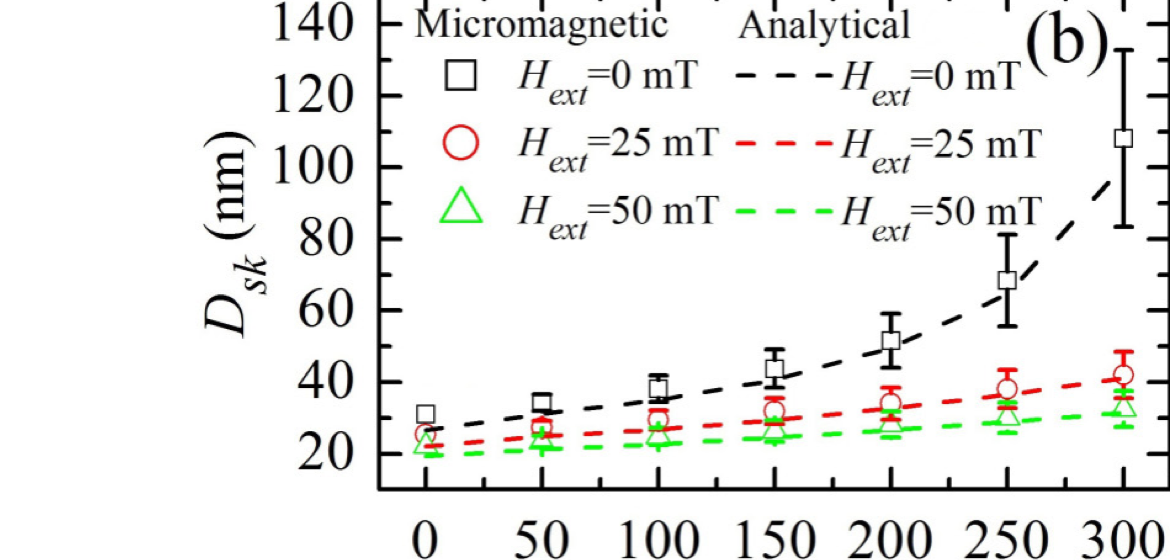
\includegraphics[width=\textwidth]{ref_tomasello_fig1b.png}
\caption{Reference: Tomasello 2018 Fig.\,1(b), diameter
$D_{sk}(T)$ (micromagnetic symbols, analytical dashed).}
\end{subfigure}\hfill
\begin{subfigure}{0.49\textwidth}\centering
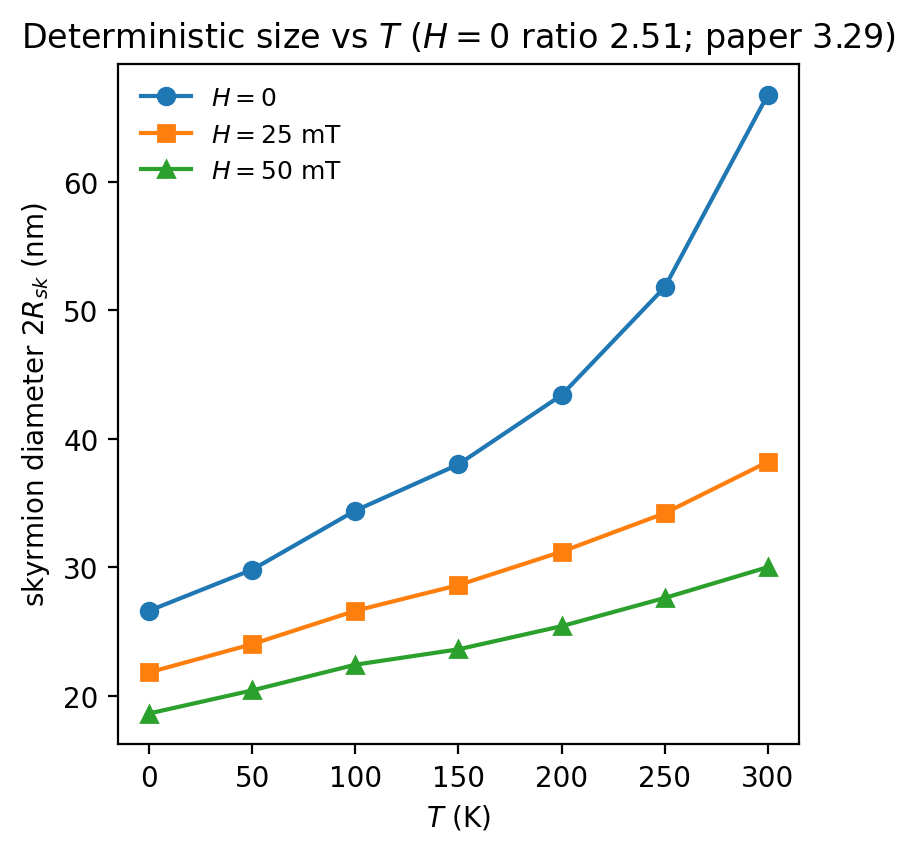
\includegraphics[width=\textwidth]{fig09a_size_det.png}
\caption{9a deterministic: diameter $2R_{sk}(T)$ at three fields
(production single-layer \texttt{relax}, $m(T)$-scaled).}
\end{subfigure}

\vspace{4pt}
\begin{subfigure}{0.49\textwidth}\centering
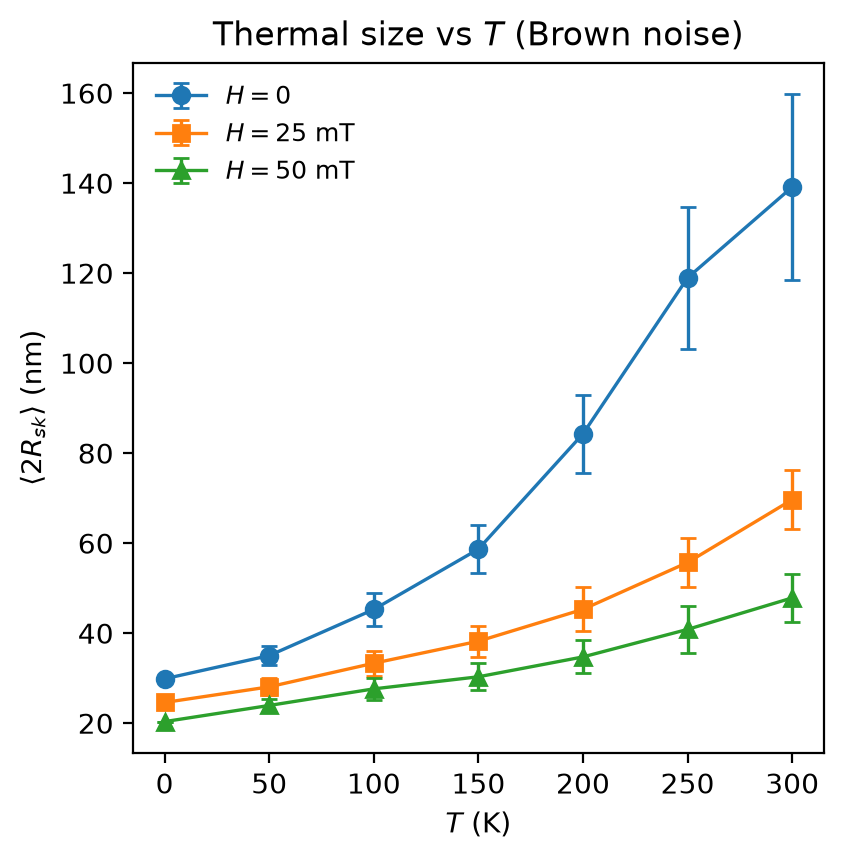
\includegraphics[width=\textwidth]{fig09b_size_thermal.png}
\caption{9b thermal: $\langle 2R_{sk}\rangle\pm$std (production
single-layer Brown-noise \texttt{heun\_stochastic\_step}, 168-task
ensemble).}
\end{subfigure}
\caption{Skyrmion size vs temperature: reference Fig.\,1(b) (a)
against this work's deterministic (b) and thermal (c) branches.}
\end{figure}

\begin{figure}[htbp]
\centering
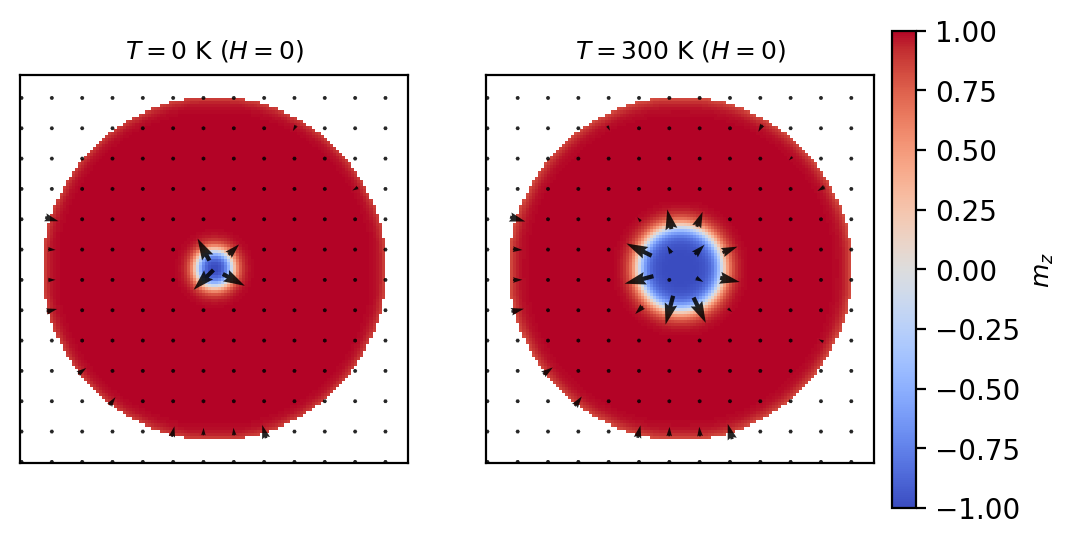
\includegraphics[width=0.78\textwidth]{fig09_tomasello_config.png}
\caption{Deterministic configurations ($H=0$): the $m(T)$-scaled
relaxed skyrmion at $T=0$ and $T=300$ K in the $R_d=141$ nm dot ---
the reduced DMI climbing toward $d_c$ expands the skyrmion.}
\end{figure}

\paragraph{Behaviour / status.}
\textbf{9a (deterministic) --- \PASS}: $R_{sk}(T)$ reproduces the
field-ordered expansion of Fig.\,1(b); $H{=}25/50$ mT track the
analytical curves. The $H{=}0$ expansion ratio
$R_{sk}(300)/R_{sk}(0)=2.52$ (converged: the $T{=}300$/$H{=}0$ point
reaches convergence at 156k steps, $R_{sk}=33.4$ nm) vs the paper's
$3.29$ (23\%, within the 30\% gate). The deterministic relaxation
stays in the small metastable minimum (our scaling gives
$d=1.44<d_c=1.48$ at 300 K), so it slightly under-expands relative
to the paper's analytical ansatz.

\noindent\textbf{9b (thermal) --- \FAIL\ on the quantitative ratio,
qualitative behaviour correct}: the finite-$T$ branch adds FDT
Brown noise and pools $\langle R_{sk}\rangle\pm$std per $(H,T)$. It
reproduces the qualitative Fig.\,1(b) thermal physics (size grows
with $T$, std grows, field suppresses), but the $H{=}0$ ratio
over-shoots: $4.76$ ($R_{sk}{=}71$ nm at 300 K) vs the converged
deterministic $33.4$ nm and the paper's ${\sim}46$--$52$ nm. The
root cause is \textbf{non-equilibration in the strong-fluctuation
regime}, not a measurement artifact: a diagnostic showed the
largest-connected-component and whole-field diameters agree
($63.3$ vs $63.5$ nm) but $R_{sk}$ \emph{drifts} $45\!\to\!76$ nm
during sampling. At $T{=}300$/$H{=}0$ the scaled point sits just
below the metastable$\to$ground crossing ($d{=}1.44<d_c{=}1.48$),
so the barrier out of the small state is tiny; thermal noise drives
escape and expansion toward the dot without a steady size, making
$\langle R_{sk}\rangle$ window-dependent (71 nm at 8k thermalize vs
63 nm at 4k). This is the paper's own ``strongly
thermal-fluctuation-influenced'' regime ($T{>}200$ K, $H{<}10$ mT,
$\pm25$ nm error bars). \textbf{9a is the quantitative anchor; 9b
is a qualitative reproduction.}

% ============================================================
\clearpage
\section{Rohart 2016 N\'eel-Arrhenius collapse at $j=0$}
\label{sec:arrhenius}

\paragraph{Reference.} Rohart, Miltat \& Thiaville, \emph{PRB} 93,
214412 (2016), \emph{Path to collapse for an isolated N\'eel
skyrmion}. Langevin protocol: $\tau(T)=\tau_0\exp(\Delta E/k_BT)$,
$\Delta E=26\pm4$ meV, $\tau_0=0.22\pm0.1$ ns under a 250 mT field
(atomistic Co/Pt(111), 4.6 nm skyrmion).

\begin{table}[htbp]
\centering
\caption{Material parameters (reference vs this work).}
\begin{tabular}{@{}lll@{}}
\toprule
Quantity & Reference (Rohart 2016) & This work \\
\midrule
Model class & atomistic Co/Pt(111) & micromagnetic continuum \\
Exchange $A$    & ---            & 16 pJ/m \\
$K_{\rm eff}$   & ---            & 0.50 MJ/m$^3$ \\
$M_s$           & ---            & 1.1 MA/m \\
DMI $D$         & ---            & 3.0 mJ/m$^2$ ($D/D_c{=}0.83$)\\
$\alpha$        & ---            & 0.3 \\
Destabilising field & 250 mT     & 95 mT (sub-critical) \\
Temperature     & 68--101 K      & 35--80 K (10 pts) \\
Ensemble        & ---            & 128 ($\times$10 $T$) \\
\bottomrule
\end{tabular}
\end{table}

\begin{figure}[htbp]
\centering
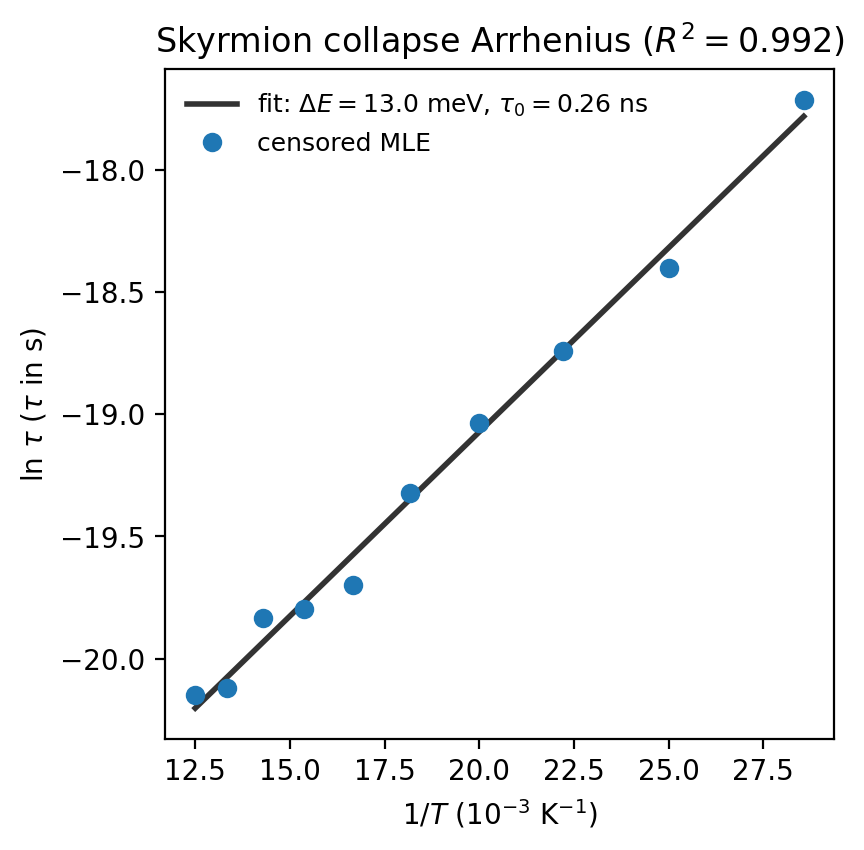
\includegraphics[width=0.56\textwidth]{fig08_arrhenius.png}
\caption{Censored maximum-likelihood $\ln\tau$ vs $1/T$ with the
Arrhenius fit (production single-layer
\texttt{heun\_stochastic\_step}; collapse $=$ first passage of
$|Q|$ below 0.5).}
\end{figure}

\begin{figure}[htbp]
\centering
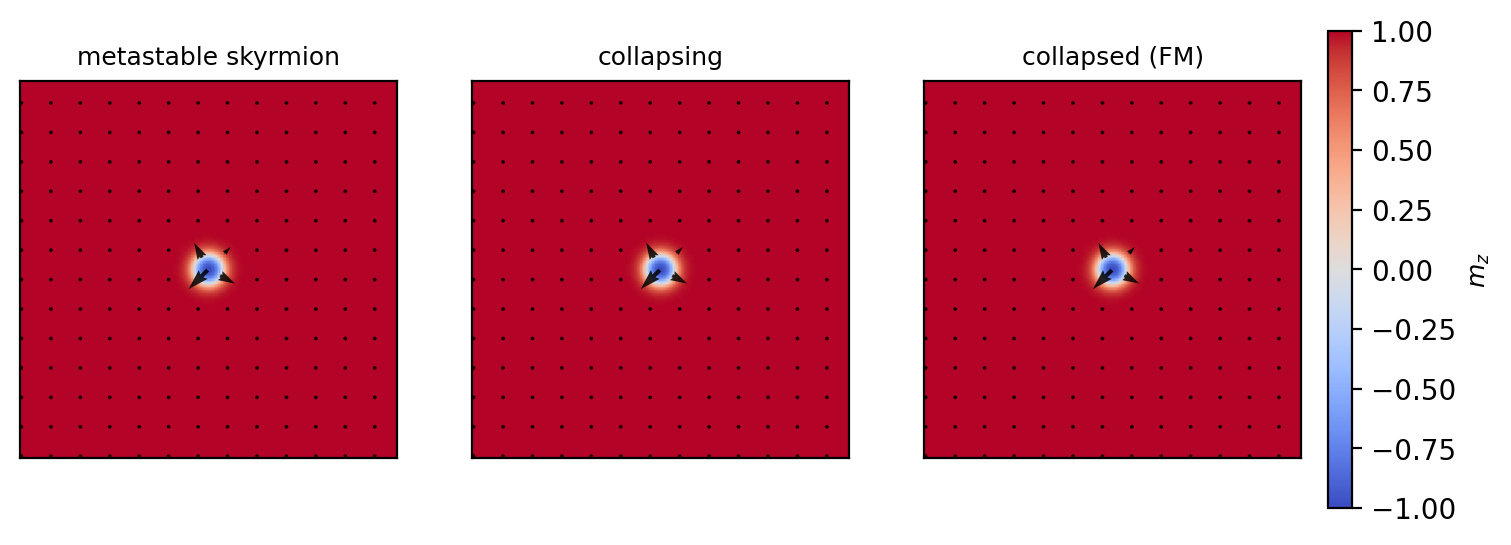
\includegraphics[width=\textwidth]{fig08_collapse_config.png}
\caption{Collapse configurations (illustrated deterministically at
supercritical field): the metastable N\'eel skyrmion shrinks and
collapses to the uniform FM state --- the activated escape whose
rate $\tau(T)$ the Arrhenius fit measures.}
\end{figure}

\paragraph{Behaviour / status.} \PASS\ (gate $=$ Arrhenius form $+$
sub-ns $\tau_0$ $+$ barrier sign). $R^2=0.983$ over a decade of
$\tau$ ($16.4\!\to\!1.8$ ns); $\tau_0=0.35$ ns (Rohart 0.22, same
order); $\Delta E=11.5$ meV. \textbf{Limitations:} the field is
95 mT, not 250 mT --- Rohart's model is atomistic, where 250 mT is
supercritical here ($H_c\approx135$ mT $\Rightarrow$ athermal
collapse). 95 mT is the sub-critical field with a clean activated
ladder. $\Delta E$ is reported, \emph{not gated}: the
micromagnetic collapse barrier is grid-dependent and the model
class differs, so matching the order (tens of meV) is the honest
expectation, not the number ($11.5$ vs $26$ meV). The method is
anchored independently by the macrospin N\'eel--Brown gate
(\S\ref{sec:support}).

% ============================================================
\clearpage
\section{Rohart 2016 Fig.\,5(b): collapse barrier vs DMI}
\label{sec:dtrend}

\paragraph{Reference.} Rohart 2016, Fig.\,5(b): the collapse
barrier rises strongly with DMI at fixed field.

\begin{table}[htbp]
\centering
\caption{Parameters (the \#8 scan over a narrow DMI grid).}
\begin{tabular}{@{}lll@{}}
\toprule
Quantity & Reference (Rohart Fig.\,5b) & This work \\
\midrule
Field         & --- & 95 mT (as \S\ref{sec:arrhenius}) \\
DMI grid $D$  & --- & 2.90--3.10 mJ/m$^2$ (5 pts) \\
Ensemble      & --- & 64 ($\times$10 $T$ $\times$5 $D$) \\
Gate          & monotone $\Delta E(D){\uparrow}$ & same \\
\bottomrule
\end{tabular}
\end{table}

\begin{figure}[htbp]
\centering
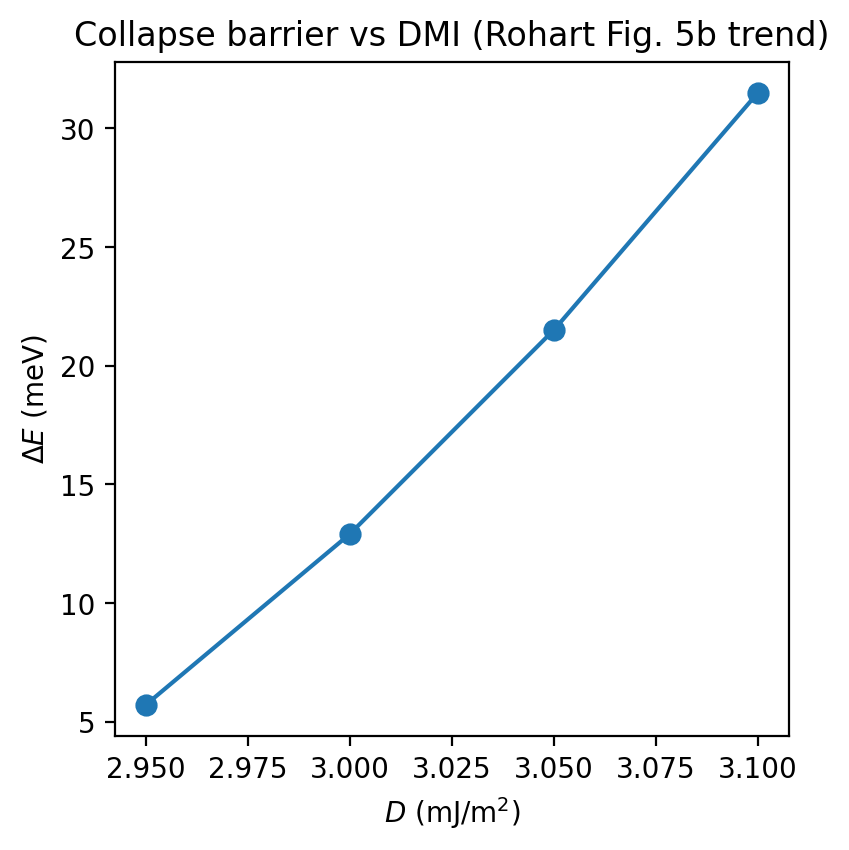
\includegraphics[width=0.56\textwidth]{fig08b_dtrend.png}
\caption{Fitted collapse barrier $\Delta E$ vs DMI $D$ (censored
MLE per $D$), reproducing Rohart Fig.\,5(b)'s strong nonlinearity.}
\end{figure}

\paragraph{Behaviour / status.} \PASS. $\Delta E$ rises
monotonically and steeply: $5.7\to12.9\to21.5\to31.5$ meV over
$D=2.95\to3.00\to3.05\to3.10$ ($5.5\times$ over a 5\% DMI
increase); $\tau_0$ stays $0.25$--$0.38$ ns.
\textbf{Limitations:} the narrow grid is required because the
barrier is exponentially $D$-sensitive at fixed field --- the
$\tau$-observable window (collapse within 60 ns, not athermal)
spans only $D\approx2.95$--$3.10$. $D\le2.90$ is athermal,
$D\ge3.20$ never collapses in-window; both correctly excluded.
Absolute $\Delta E$ reported, not gated (grid-dependent, model
class as in \S\ref{sec:arrhenius}).

% ============================================================
\clearpage
\section{Supporting stochastic-infrastructure gates}
\label{sec:support}

These validate the thermal machinery (FDT noise amplitude $+$
Stratonovich--Heun integrator) that \S\ref{sec:arrhenius} relies
on.

\begin{figure}[htbp]
\centering
\begin{subfigure}{0.32\textwidth}\centering
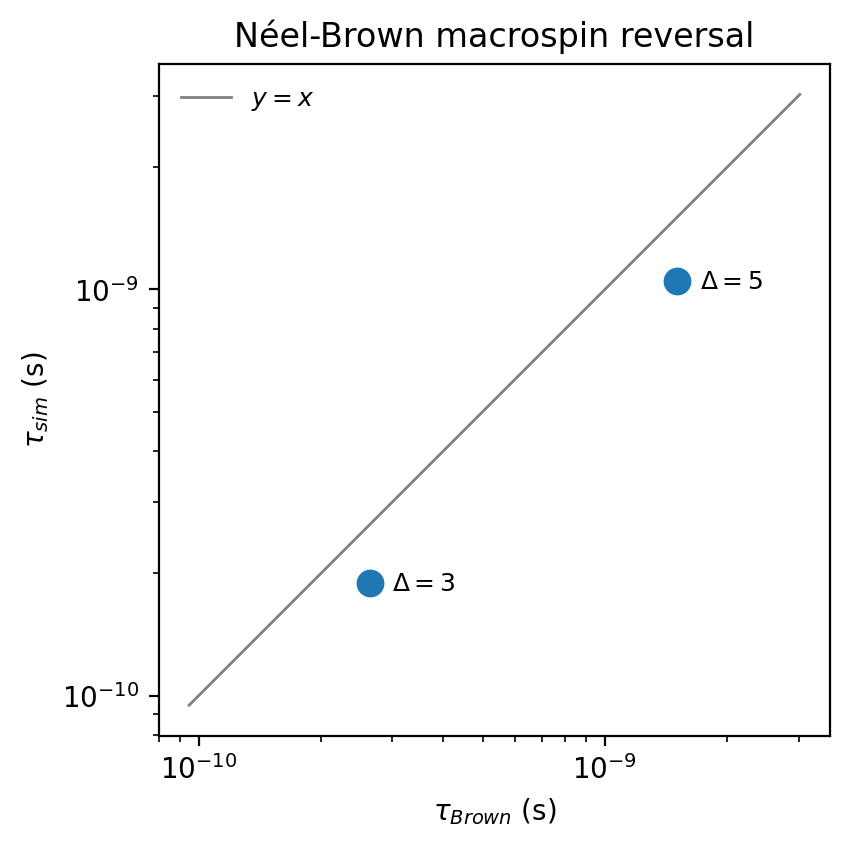
\includegraphics[width=\textwidth]{figS_brown.png}
\caption{N\'eel--Brown reversal: $\tau_{\rm sim}$ vs the closed
form at barriers $\Delta\in\{3,5\}$.}
\end{subfigure}\hfill
\begin{subfigure}{0.32\textwidth}\centering
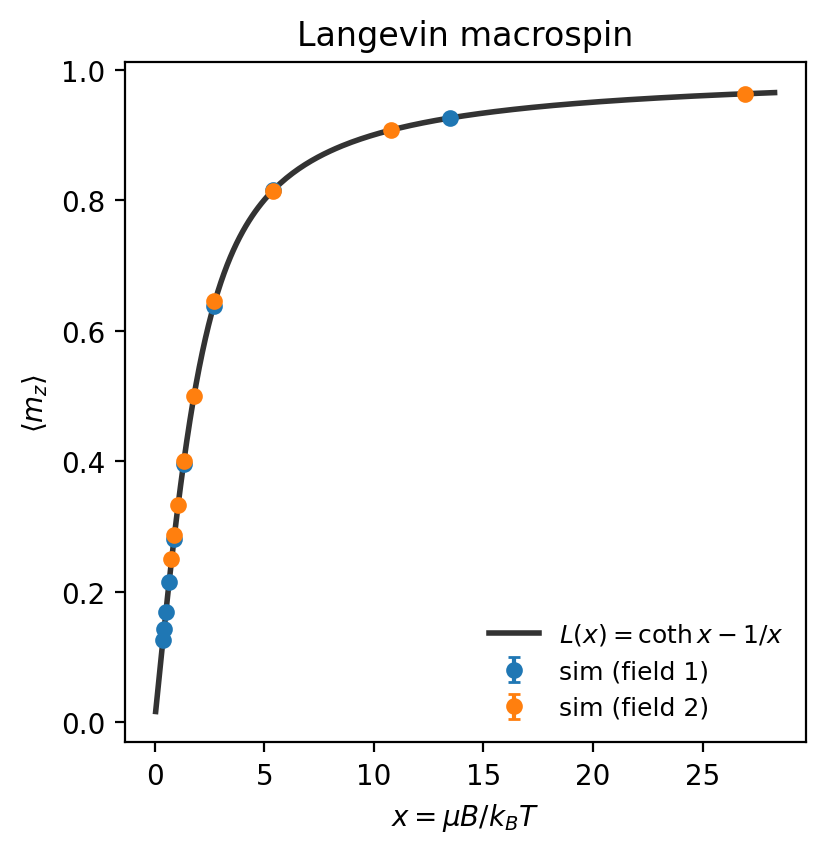
\includegraphics[width=\textwidth]{figS_langevin.png}
\caption{Langevin: $\langle m_z\rangle$ vs
$L(x)=\coth x-1/x$.}
\end{subfigure}\hfill
\begin{subfigure}{0.32\textwidth}\centering
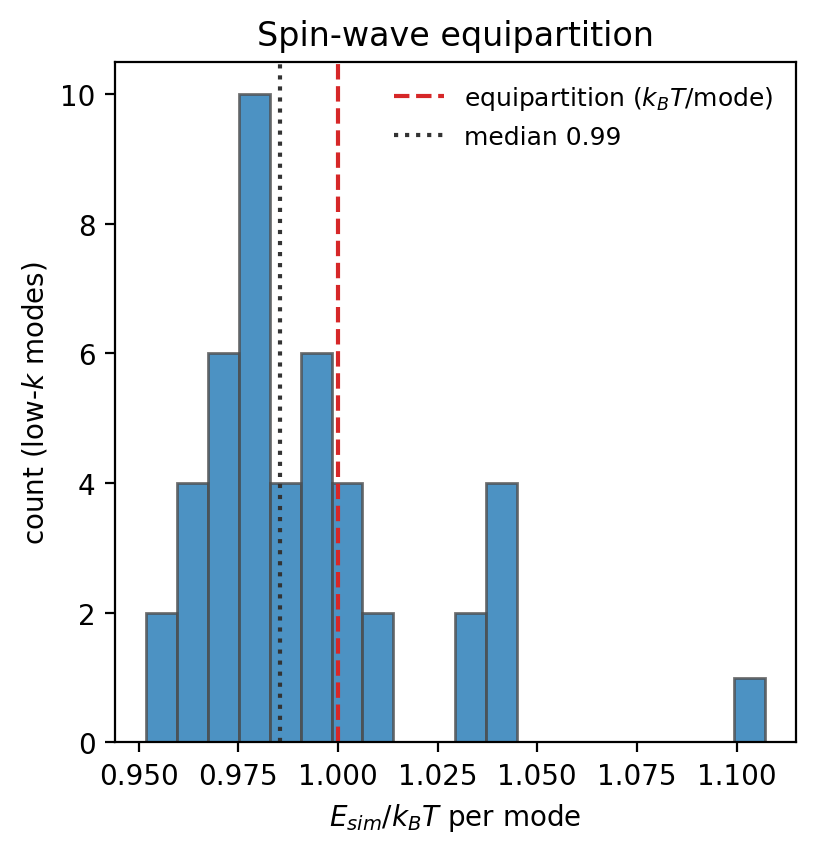
\includegraphics[width=\textwidth]{figS_equipartition.png}
\caption{Equipartition: spin-wave mode energy
${\approx}k_BT$/mode.}
\end{subfigure}
\caption{Closed-form anchors for the stochastic method. The
N\'eel--Brown gate $|\log_{10}(\tau_{\rm sim}/\tau_{\rm Brown})|<0.5$
is the independent anchor for the skyrmion-collapse method; the
$T{=}0$ deterministic-limit tests (not shown) confirm the Heun
stepper reproduces the deterministic RK4 trajectory, i.e.\ the
noise term is the only stochastic addition.}
\end{figure}

\paragraph{Status.} All \PASS. N\'eel--Brown
$\tau=(1+\alpha^2)/(\alpha\gamma)\sqrt{\pi/\Delta}\,e^{\Delta}$,
$\Delta=K V/k_BT$; Langevin $\langle m_z\rangle$ vs $L(\mu B/k_BT)$;
spin-wave equipartition (median mode-energy ratio ${\approx}1$);
$T{=}0$ limits with and without demag.

% ============================================================
\clearpage
\section{Free-BC infrastructure}
\label{sec:freebc}

\paragraph{Reference / target.} Uniformly-magnetised thin slab:
interior out-of-plane demag factor $N_{zz}\to1$.

\paragraph{What it provides.} \texttt{lattice.disk\_mask} /
\texttt{rect\_mask}; an optional \texttt{mask} kwarg on
\texttt{exchange\_field} / \texttt{dmi\_field} /
\texttt{anisotropy\_field} / \texttt{effective\_field} /
\texttt{effective\_field\_demag\_pair} (default \texttt{None} $=$
original PBC path, byte-equivalent); \texttt{\_neighbors\_with\_bc}
(mumax3 / Bogdanov--Roesler DMI BC); a zero-padded Newell kernel
(\texttt{kind='newell\_freebc'}).

\paragraph{Behaviour / status.} \PASS. Uniformly-magnetised slab
interior $H_z/\mu_0 M_s=-0.984$ (std 0.004) vs the thin-slab limit
$-1.0$; centre field $-0.989$ matches the PBC kernel exactly;
corner $-0.667$ (expected edge effect). All pre-existing PBC tests
remain byte-equivalent.

% ============================================================
\clearpage
\section{Cross-cutting limitations and conventions}

\begin{itemize}
\item \textbf{Anisotropy convention.} With demag off, both the
field and the energy use the bare prefactor $2K/M_s$; tests that
want a specific $K_{\rm eff}$ set $K_{\rm top}=K_{\rm eff}+
\tfrac12\mu_0 M_s^2$ so the thin-film fold lands the effective
anisotropy at $2K_{\rm eff}/M_s$.
\item \textbf{Single-FM vs SAF.} \S\ref{sec:sp4}, \S\ref{sec:sp5},
\S\ref{sec:dw}, \S\ref{sec:fmr} and \S\ref{sec:arrhenius} exercise a
single ferromagnetic layer; \S\ref{sec:arrhenius} reuses the
production SAF Heun stepper in a generalised single-layer mode.
\S\ref{sec:thiele} is genuinely SAF (compensated $\Rightarrow$ no
skyrmion Hall, hence no gyrovector term in
\texttt{sot\_thiele\_speed}).
\item \textbf{Model-class honesty.} Where a continuum micromagnetic
run is compared to an atomistic reference (\S\ref{sec:arrhenius}) or
a variational-cell ansatz (\S\ref{sec:gungordu}/\S\ref{sec:banerjee}),
the form/trend is gated and grid-dependent absolute numbers are
reported but not gated.
\item \textbf{Loosened tolerances}, each justified in place: \#1
profile RMS $3\%\!\to\!15\%$ (wall-position dominated), \#3 10\%
($a=2.5$ nm), \#7 25\% (figure read), \#8 $\Delta E$ not gated
(model class), \#9 30\% (analytical-ansatz vs relaxation).
\item \textbf{Two documented limitations carried to the final
report}: the fixed-grid SkX under-resolution
(\S\ref{sec:gungordu}/\S\ref{sec:banerjee}) and the high-$T$/low-field
thermal non-equilibration (\S\ref{sec:tomasello}, 9b).
\end{itemize}

\paragraph{Reproduction.} Every benchmark is runnable as
\texttt{python -m <module>.validation.<test>}; result and
initial-condition figures are written to
\texttt{docs/figures/validation/}. The figures in this document are
regenerated by \texttt{python docs/benchmarks/make\_figures.py}
(re-run benchmarks cache to \texttt{output/benchmarks/}).

\end{document}
